\chapter{Data Analysis}

\section{Overview}



This analysis is motivated by the GGM supersymmetry breaking scenario in which the strong production of either gluinos or squarks result in a final state containing two photons, jets, and missing transverse momentum.  Two example topologies are shown in Figure \ref{fig:susysignals}.  In the T5gg model, each of the produced gluinos decays to a neutralino which then decays to a photon and a gravitino.  Similarly, the T6gg model has each of the produced squarks decays to a neutralino which then decays to a photon and a gravitino.  In both cases the gravitino escapes the CMS without detection which manifests as missing transverse momentum.  

\begin{figure}[h]
	\centering
	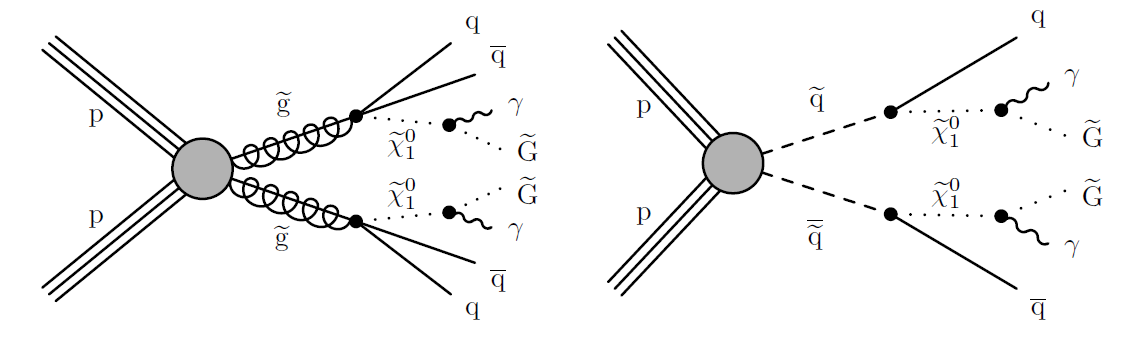
\includegraphics[width=0.9\linewidth]{Figures/SUSYsignals}
	\caption{Two examples of GGM supersymmetry breaking processes resulting in final states conaining two photons and missing transverse momentum. The T5gg model (left) shows gluinos produced from $p-p$ collisions which subsequently result in two neutralinos, each decaying to a photon and a gravitino. The T6gg model (right) shows squarks produced from $p-p$ collisions following a similar decay chain.}
	\label{fig:susysignals}
\end{figure}


\section{Data}
This analysis was performed using 137 fb$^{-1}$ of data collected from the CMS detector during the time period commonly referred to as Run 2 which spans from  2016 to 2018.  The complete list of the datasets used can be found in Table \ref{table:DataSamples}.  The JSON files used to identify events passing all of the CMS offline data quality monitoring requirements are:

\begin{verbatim}
	Cert_271036 284044_13TeV_23Sep2016ReReco_Collisions16_JSON.txt
	Cert_294927 306462_13TeV_EOY2017ReReco_Collisions17_JSON_v1.txt 
	Cert_314472 325175_13TeV_PromptReco_Collisions18_JSON.txt 
\end{verbatim} 

\begin{table}[h!]
	\centering
	\caption{Data Samples}
	\begin{tabular}{|c|}
		\hline
		/DoubleEG/Run2016B-17July2018-ver2-v1 \\
		\hline
		/DoubleEG/Run2016C-17July2018-v1 \\
		\hline
		/DoubleEG/Run2016D-17July2018-v1 \\
		\hline
		/DoubleEG/Run2016E-17July2018-v1 \\
		\hline
		/DoubleEG/Run2016F-17July2018-v1 \\
		\hline
		/DoubleEG/Run2016G-17July2018-v1 \\
		\hline
		/DoubleEG/Run2016H-17July2018-v1 \\
		\hline
		/DoubleEG/Run2017B-31Mar2018-v1 \\
		\hline
		/DoubleEG/Run2017C-31Mar2018-v1 \\
		\hline
		/DoubleEG/Run2017D-31Mar2018-v1 \\
		\hline
		/DoubleEG/Run2017E-31Mar2018-v1 \\
		\hline
		/DoubleEG/Run2017F-31Mar2018-v1 \\
		\hline
		/EGamma/Run2018A-17Sep2018-v2 \\
		\hline
		/EGamma/Run2018B-17Sep2018-v1 \\
		\hline
		/EGamma/Run2018C-17Sep2018-v1 \\
		\hline
		/EGamma/Run2018D-22Jan2019-v2 \\
		\hline
	\end{tabular}
	\label{table:DataSamples}
\end{table}

\section{Monte Carlo samples}
Monte Carlo (MC) simulation were used to validate performance of the analysis on backgrounds, model background contributions, constructing a multivariate discriminant, and determining signal efficiencies.   The MC samples used for this analysis are listed in Table \ref{table:MCSamples}.
\begin{table}
	\centering
	\caption{Table of MC samples used.}
	\begin{tabular}{|l|l|}
		\hline
		Sample name & Purpose \\
		\hline
		\hline
		GJets & Training MVA discriminate for QCD background \\
		\hline
		ZGGToNuNuGG & Prediction of irreducible $Z\gamma \gamma \rightarrow \nu \nu \gamma \gamma$ background \\
		\hline
		ZGGToLLGG & Renormalization of $Z\gamma \gamma \rightarrow \nu \nu \gamma \gamma$ background \\
		\hline
		TTJets & Testing EWK background prediction method\\
		\hline
	\end{tabular}
	\label{table:MCSamples}
\end{table}

The distribution of pileup (PU) interactions produced in simulated events differs from data.  Since the presence of additional PU interactions affects many aspects of reconstruction, it's important for the PU to be properly simulated.  To correct for these differences between MC and data the simulated events are reweighted so that the PU profile in MC matches the profile in data.  In MC the PU is number of simulated vertices in an event while the PU in data is calculated by the method discussed in Section \ref{section:pucorrection}.  
  

\section{Object definitions}
The object candidates that are identified by the reconstruction algorithms are subject to further scrutiny in order to achieve optimal purities in the offline analysis.  

\subsection{Photons}
Photons are required to have $p_T>80$ GeV and meet the criteria prescribed by loose ID cuts derived by the $e/\gamma$ Physics Object Group (EGM POG).  The cut variables used to determine the photon ID are:

\begin{itemize}
	\item H/E - The ratio of the energy deposited in the HCAL tower that is directly behind the ECAL supercluster associated with the photon to the energy deposited in the ECAL supercluster.
	\item $\sigma_{i\eta i\eta}$ - The log-fractional weighted width of a shower in $i\eta$-space.  This variable is used to describe the shower shape or more specifically it provides a measure of the spread of the shower in the $\eta$-direction.  The log-fractional weight is the log of the ratio of energy deposited in a specific ECAL crystal versus the energy deposited in the associated $5\times 5$ supercluster.
	\item Particle Flow Charged Isolation - Sum of the $p_T$ of charged hadrons associated with the primary vertex within a cone of $0.02 < \Delta R < 0.3$ of the supercluster.
	\item Particle Flow Neutral Isolation - Sum of the $p_T$ of neutral hadrons associated with the primary vertex within a cone of $\Delta R < 0.3$ of the supercluster.
	\item Particle Flow Photon Isolation - Sum of the $p_T$ of photons within a cone of $\Delta R < 0.3$ of the supercluster.
\end{itemize}

All of the isolation variables listed above are corrected in order to remove pileup as described in Section \ref{section:pucorrection}.  Table \ref{table:looseIDPhotonreq} gives a summary of the pileup-corrected requirements for a loose ID photon.  The loose ID working point has an efficiency (background rejection) of $90.08\%$ ($86.25\%$) in the barrel and $90.65\%$ ($76.72\%$) in the end caps.  In addition to the $p_T$ and loose ID requirements, a photon must also pass a pixel seed veto (PSV).  This means that there is no pixel seed in the tracker matched to the photon.

\begin{table}[h]
	\centering
	\caption{Summary of loose ID photons cuts}
	\begin{tabular}{|l|l|l|}
		\hline
		Variable & Cut Value (Barrel) & Cut Value (Endcap) \\
		\hline
		H/E & 0.04596 & 0.0590 \\
		\hline
		$\sigma_{i\eta i\eta}$ & 0.0106 & 0.0272 \\
		\hline
		Charged Iso & 1.694 & 2.089 \\
		\hline
		Neutral Iso & $24.032 + 0.01512 p_{T\gamma} + 2.259\times 10^{-5}p^2_{T\gamma}$ & $19.722 + 0.0117 p_{T\gamma} + 2.3\times 10^{-5}p^2_{T\gamma}$ \\
		\hline
		Photon Iso & $2.876 + 0.004017 p_{T\gamma}$ & $4.162 + 0.0037 p_{T\gamma}$ \\
		\hline
	\end{tabular}
	\label{table:looseIDPhotonreq}
\end{table}

Photon ID efficiencies differ between data and MC, so when using a photon ID in MC samples we scale them by a "scale factor" (SF) in order to replicate detector efficiencies for that that particular ID.  The loose photon ID efficiency is measured using the tag-and-probe method on $Z\rightarrow ee$ events in both data and MC.  The probe is chosen to be one of the electrons while the other electron is used as the tag.  The ratio of how many probes pass the loose photon ID requirements and the total number of tag and probe pairs gives the efficiency $\epsilon$ for the loose photon ID.  We then define the SF as the data efficiency divided by the efficiency in MC or $SF = \frac{\epsilon_{data}}{\epsilon_{MC}}$.  Applying the SF to MC events essentially removes the MC efficiency and replaces it with the real detector efficiency to give
\begin{equation}
	N_{obs} = N_{gen}\cdot \epsilon_{MC}\cdot SF =  N_{gen}\cdot \epsilon_{MC}\cdot \frac{\epsilon_{data}}{\epsilon_{MC}} = N_{gen}\cdot \epsilon_{data}.
\end{equation}
Since this analysis requires two loose ID photons, the scale factor $SF$ is given by the product of scale factors for each of the two loose photons, $SF = SF_{\gamma1}\cdot SF_{\gamma2}$.  The scale factors for each year are shown in Figures \ref{fig:loosephotonsf2016}, \ref{fig:loosephotonsf2017}, and \ref{fig:loosephotonsf2018} in bins of photon $p_T$ and $\eta$ \cite{PhotonSF}.
\begin{figure}[h]
	\centering
	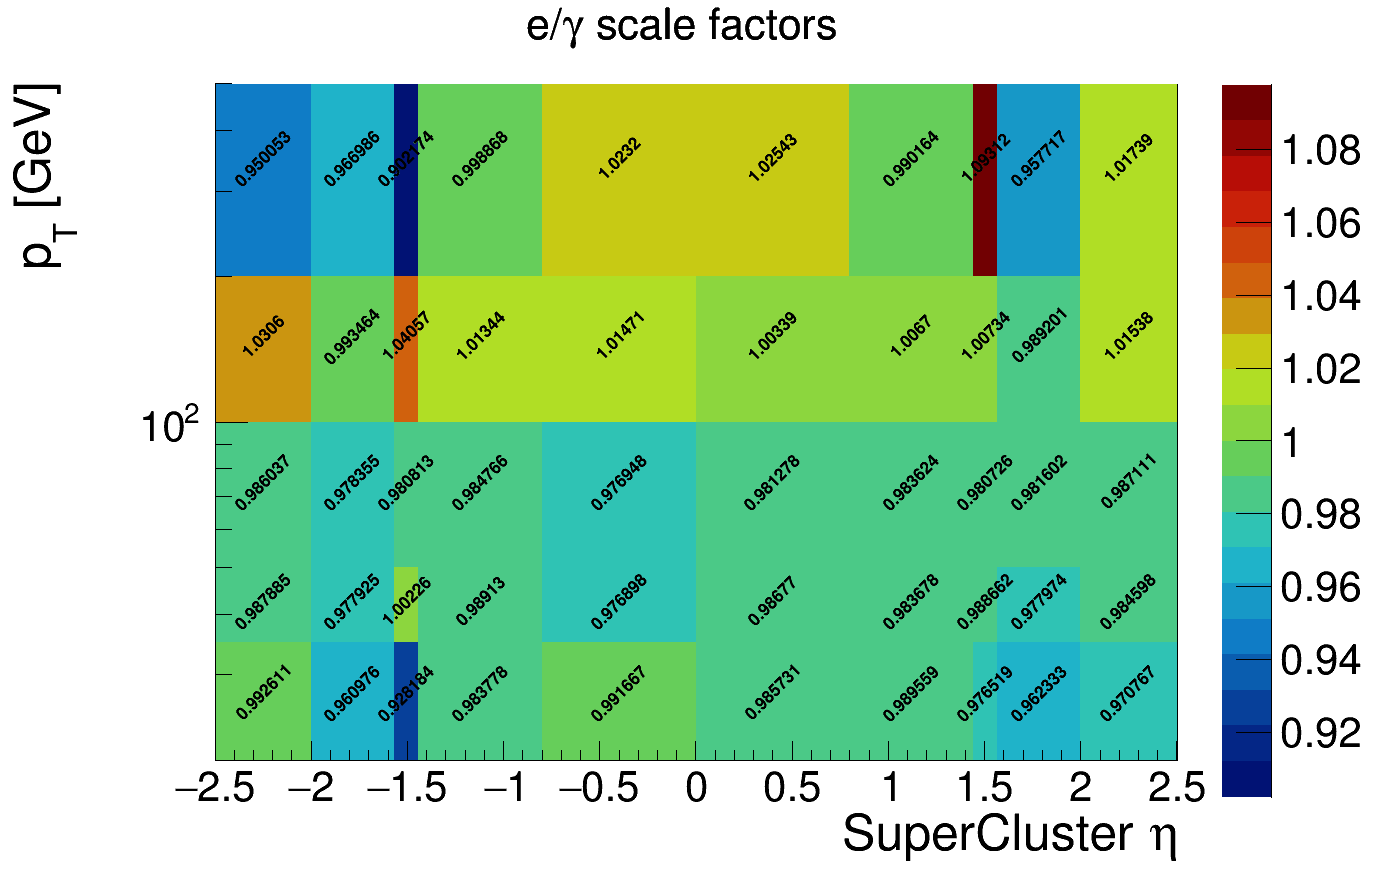
\includegraphics[width=1.0\linewidth]{Figures/LoosePhotonSF_2016}
	\caption[Scale factors for 2016 loose photon ID.]{The loose photon ID scale factors for 2016 in bins of photon $p_T$ and $\eta$}
	\label{fig:loosephotonsf2016}
\end{figure}
\begin{figure}[h]
	\centering
	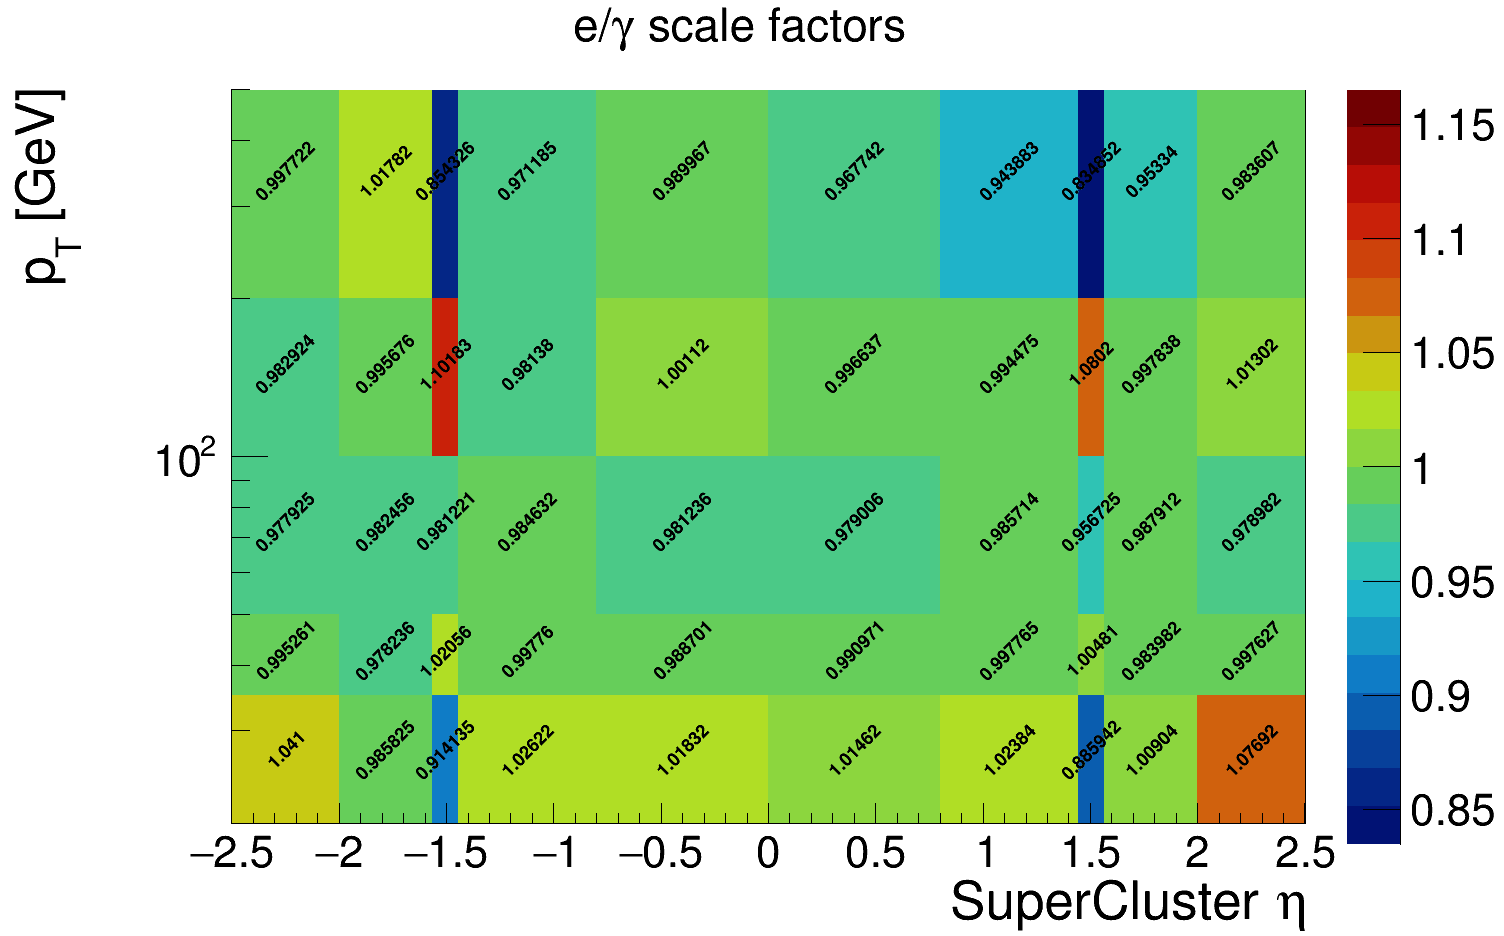
\includegraphics[width=1.0\linewidth]{Figures/LoosePhotonSF_2017}
	\caption[Scale factors fo 2017 loose photon ID.]{The loose photon ID scale factors for 2017 in bins of photon $p_T$ and $\eta$.}
	\label{fig:loosephotonsf2017}
\end{figure}
\begin{figure}[h]
	\centering
	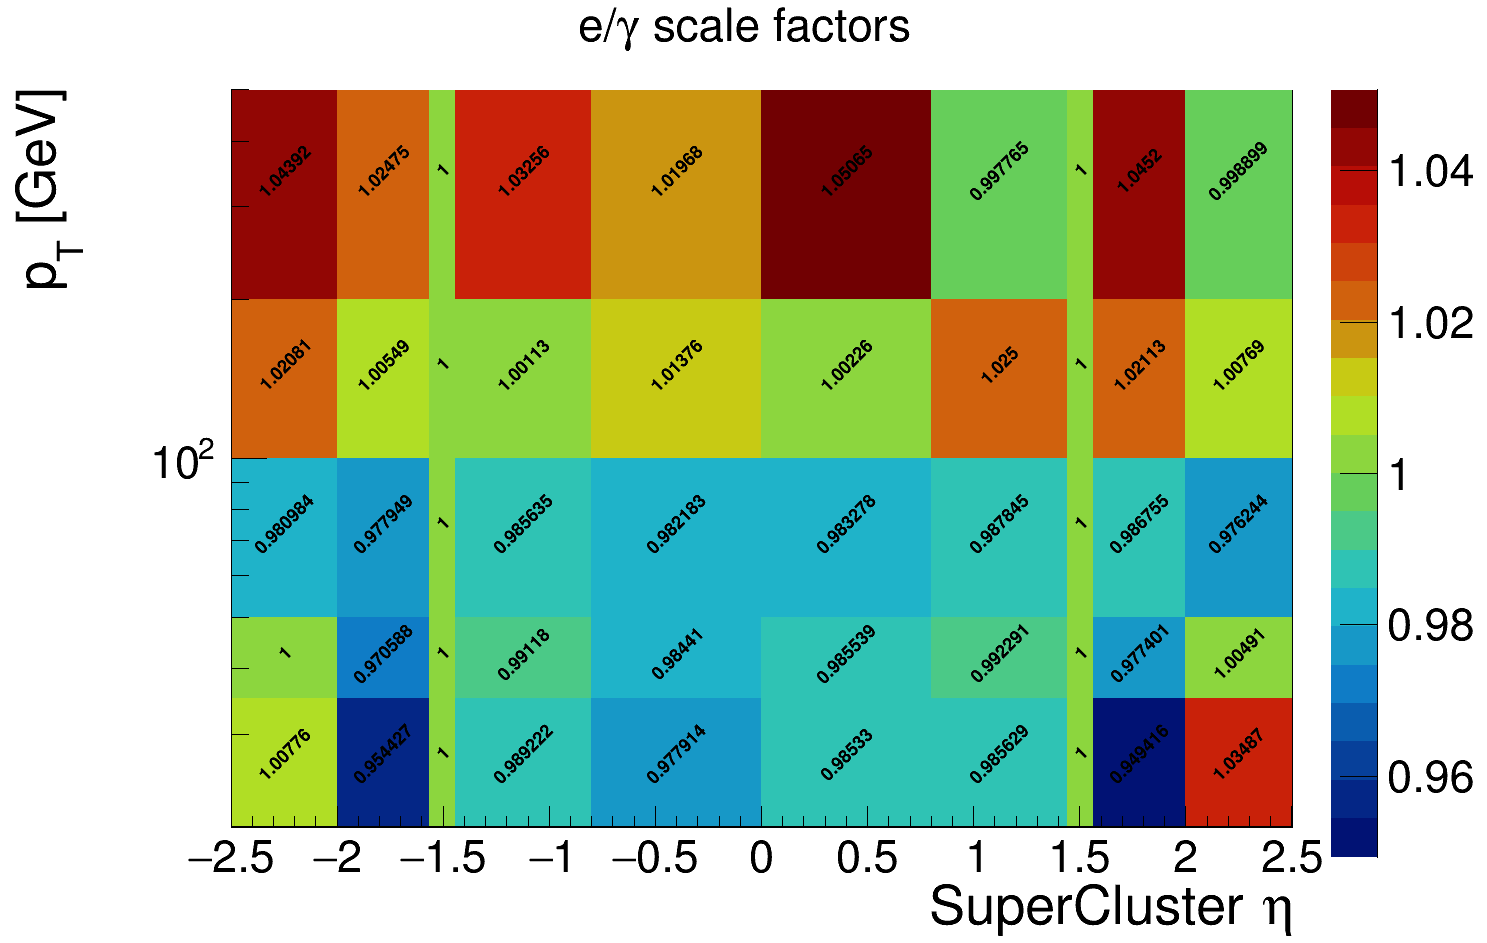
\includegraphics[width=1.0\linewidth]{Figures/LoosePhotonSF_2018}
	\caption[Scale factors for 2018 loose photon ID.]{The loose photon ID scale factors for 2018 in bins of photon $p_T$ and $\eta$.}
	\label{fig:loosephotonsf2018}
\end{figure}


\label{section:photondefinition}

\subsection{Electrons}
As mentioned earlier, the clustering algorithm doesn't differentiate between showers from photons and those from electrons.  In this analysis an electron is defined as an object that passes all of the photon requirements except for the PSV.  Inverting the pixel seed requirement while using the same ID criteria ensures that we have orthogonal selections while minimizing the bias potentially introduced by using control regions with electrons to model diphoton signal regions.  This essentially allows us to group photons and electrons together to be treated as electromagnetic objects and then splitting those objects into photon and electron objects depending on whether or not there is a pixel seed associated with it.


\subsection{Muons}
Muons are required to have $p_T > 30$ GeV, $|\eta|<2.4$, and pass the medium ID requirements listed below \cite{Sirunyan_2018}:
\begin{itemize}
	\item Must be identified by PF algorithm as either a tracker or a global muon.
	\item At least 80\% of the inner tracker layers traversed by a track must have recorded hits.
	\item If it's only reconstructed as a tracker muon, the muon segment compatibility must be > 0.451.
	\item If it's reconstructed as both a tracker and a global muon:
	\begin{itemize}
		\item the muon segment compatibility must be > 0.303
		\item the global fit must have a goodness-of-fit per degree of freedom  ($\chi^2$/dof) < 3
		\item the $\chi^2$ of the position match between standalone muon and the tracker muon must be < 12
		\item the kink-finding algorithm must give a maximum $\chi^2$ that is < 20
	\end{itemize}
\end{itemize}		
The types of muons (global, tracker, and standalone) are those described in Chapter \ref{section:muondefinitions}.  The medium ID criteria results in an efficiency of > 98\% for muons with $p_T > 20$ GeV \cite{MuonIDPerf}.

\subsection{Jets}
Jets are reconstructed using the anti-k$_T$ algorithm described in Chapter \ref{section:jetalgorithm} within a cone having radius $R = 0.4$.  

The nature of this reconstruction also labels the previously mentioned objects (photons, electrons, and muons) as jets so these need to be removed from the jet collection in order to leave us with only hadronic jets.  This process is called "cleaning" the jets. 

Still working on this section...

\label{section:jetdefinition}

\section{Event selection}
Candidate events are required to pass the following requirements:
\begin{itemize}
	\item Number of loose photons without a pixel seed requirement $\geq 2$
	\item Number of hadronic jets $\geq 2$
	\item Hard $E_T^{miss} \geq 130$ GeV
	\item Pass HLT
	\item Pass relevant event filters recommended by various POGs
\end{itemize}
The event filters mentioned above are designed to reject events with instrumental anomalies such as noise and beam backgrounds.  These filters are:
\begin{itemize}
	\item globalSuperTightHalo2016Filter
	\item HBHENoiseFilter
	\item HBHEIsoNoiseFilter
	\item eeBadScFilter
	\item BadChargedCandidateFilter
	\item BadPFMuonFilter
	\item CSCTightHaloFilter
	\item EcalDeadCellTriggerPrimitiveFilter
	\item ecalBadCalibReducedExtraFilter
	\item ecalBadCalibReducedFilter
	\item Good vertex filter (requiring at least one good reconstructed vertex)
\end{itemize}

\section{Backgrounds}
The sources of background in this analysis can be grouped into three categories.  In order of decreasing contribution they are mismeasured hadronic activity, electrons misidentified as photons, and standard model processes having final states with neutrinos and two photons.  In events with multiple jets, limitations on the jet energy resolution can give rise to an apparent imbalance in $p_T$ as is shown in Figure \ref{fig:fakemet}.  Such events are usually from quantum chromodynamics (QCD) processes.  In these cases jets can be misidentified as photons or there can be real photons being produced.  In both cases the result is the appearance of two photons accompanied by $E^{miss}_T$ which mimics our signal.  Given the large cross-section for QCD, this is the most significant background in this analysis.  The next background, resulting from the misidentification of electrons as photons, comes from electroweak (EWK) processes, in particular $W\gamma$ and $W + jets$ events where $W \rightarrow e\nu$.  Here the neutrino contributes real $E^{miss}_T$ while the fake photon allows this event to fulfill the diphoton requirement.  The final background is from $Z\gamma \gamma \rightarrow \nu \nu \gamma \gamma$ events, which exactly mimic our signal, and is modeled using simulation as it is irreducible.

\begin{figure}
	\centering
	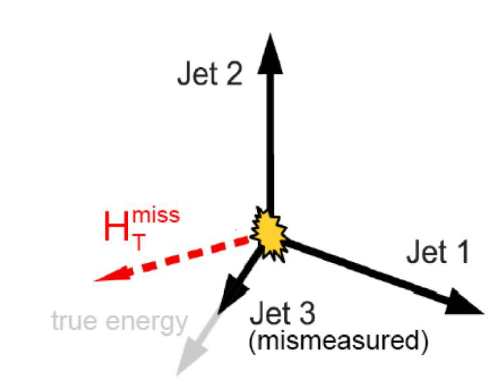
\includegraphics[width=0.5\linewidth]{Figures/FakeMET}
	\caption{Mismeasurement of Jet3 results in an inbalance in the events transverse momentum.}
	\label{fig:fakemet}
\end{figure}

\subsection{Instrumental background}
The instrumental background is the contribution from events with spurious $E^{miss}_T$ due to mismeasured hadronic activity.  The vast majority of interactions produced from proton-proton collisions at the LHC are hadronically rich QCD events.  Aside from some very rare final states with heavy-flavor jets, these events do not include neutrinos, which are the only stable particles in the SM that pass through the CMS detector unobserved, and therefore exhibit little or no $E^{miss}_T$ at the parton level.  However, the measurements of final-state particles are made using the tracker and calorimeters which have finite energy and momentum resolution.  These limitations propagate into the calculation of $E^{miss}_T$ leading to an inequality between the real, parton level $E^{miss}_T$ in an event and the measured $E^{miss}_T$.  Since most of this background is comprised of QCD events, it is commonly referred to as the "QCD background" and those terms are used interchangeably in this thesis.  Modeling of this background was done using the Rebalance and Smear technique while a multivariate discriminant was constructed to improve the efficiency of identifying events with fake $E^{miss}_T$.

\subsubsection{Rebalance and Smear}
%The Rebalance and Smear method is used to model the spurious $E^{miss}_T$ background.  The general idea is to rebalance the collection of measured jets such that it reproduces what is seen at the parton level and then smear the rebalanced jets in a way consistent with the known jet energy resolutions to return the rebalanced event to a more detector-like event.

%Coming soon....

%To estimate the QCD background, the Rebalance and Smear method is used.  This method makes use of a jet energy response model of the CMS detector and a prior probability distribution function of the particle-level Hard $E_T^{miss}$ in QCD events.  A seed sample is obtained by selecting real events from data according the baseline selection but removing the requirement on the Hard $E_T^{miss}$.  Each event in the seed sample is unfolded to produce a pseudo generator-level QCD event, or \textit{rebalanced} event.  The unfolding is carried out by rescaling the energy of each jet to a configuration that maximizes a posterior density based that is based on the jet response model.  This procedure is referred to as the \textit{rebalance} step.  The \textit{smear} step then smears the energies of all of the rebalanced jets in the event according to a random sampling of jet energy response.  This method has been developed in the context of QCD background estimation for several previous SUSY searches in the all-hadronic channel.  It has been developed here to accommodate the presence of photons and other particles in the event who's energy is the event is measured more accurately than that of jets.  This was done by fixing the 4-vectors of all of these particles during both the rebalance and smear steps so that only the jet energies are allowed to float in the maximization.


To estimate the QCD background, the Rebalance and Smear method is used.  The first step in this method is to \textit{rebalance} events such that the $E_T^{miss}$ is removed from the event to create a set of seed event.  In the second step all of the jets are \textit{smeared} with the full jet response function, which is obtained from the jet response discussed in Section \ref{section:jetalgorithm}.  This creates a set of seed events which are used in the second step to \textit{smear} all of the jets with the full jet response function to create events that model the detector response to multi-jet final states.  Figure This method has been developed in the context of QCD background estimation for several previous SUSY searches in the all-hadronic channel \cite{Goebel:2015kca}, \cite{RandS:2017abv}.  It has been developed here to accommodate the presence of photons and other particles in the event who's energy is measured more accurately than that of jets.  This was done by fixing the 4-vectors of all of these particles during both the rebalance and smear steps so that only the jet energies are allowed to float in the maximization.
\begin{figure}[h]
	\centering
	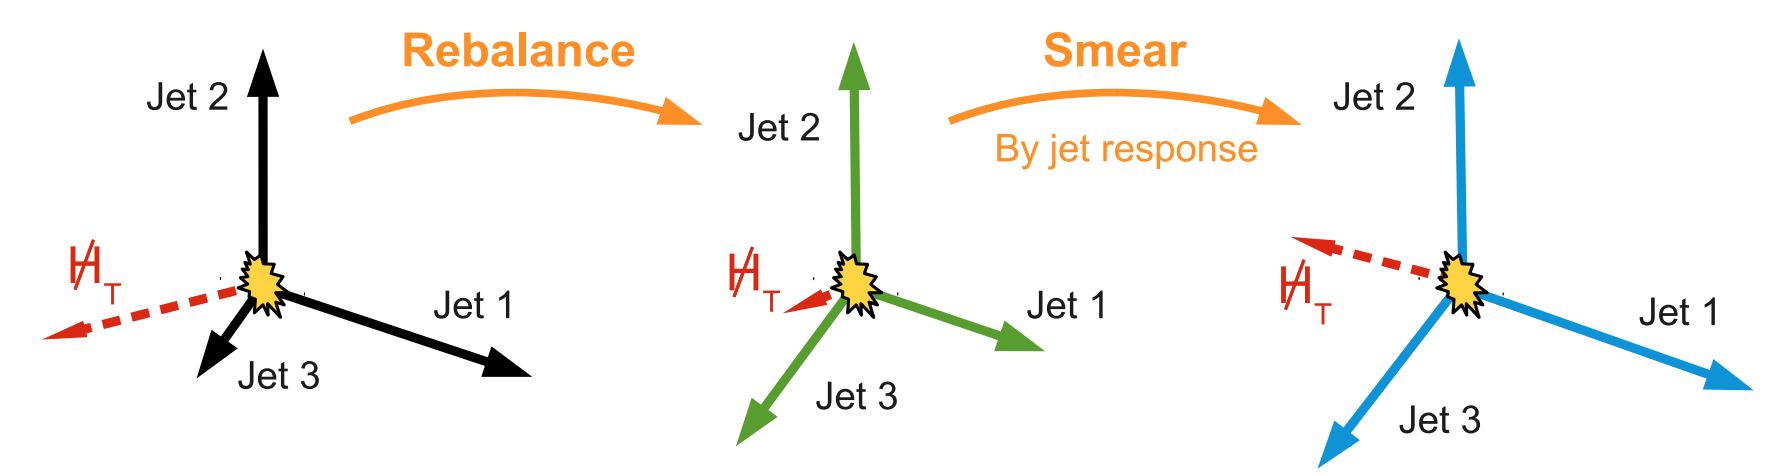
\includegraphics[width=1.0\linewidth]{Figures/RandScartoon}
	\caption[Summary of the steps for the Rebalance and Smear method.]{Summary of the steps in the Rebalance and Smear method.  The diagram shown here is for an all-hadronic final state and therefore uses hadronic missing transverse energy $\cancel{H}_T$ which is synonymous with $E_T^{miss}$ in this case\cite{Goebel:2015kca}.}
	\label{fig:randscartoon}
\end{figure}

The rebalancing in the first step is performed based on a kinematic fit \cite{DHondt:2006iej}, which is a least-square fit of the jet energies in the event while taking into account the jet response function.  When performing the fit, it is assumed that in each event the kinematic constraints of conservation momentum are fulfilled, i.e. the total $\vec{p_T}$ in the event is balanced.  Figure \ref{fig:rebalancedjetres} shows a comparison of the jet energy response $\mathcal{R} = \frac{p_T}{p_T^{gen}}$ between leading jets in QCD MC events having $E_T^{miss}>120$ GeV before and after rebalancing of the event.  We see that rebalancing has the effect of improving the jet energy resolution, which is the width of this distribution as discussed in \ref{section:jetalgorithm}, and also recovering some of the energy that was lost in the original jet reconstruction.
\begin{figure}[h]
	\centering
	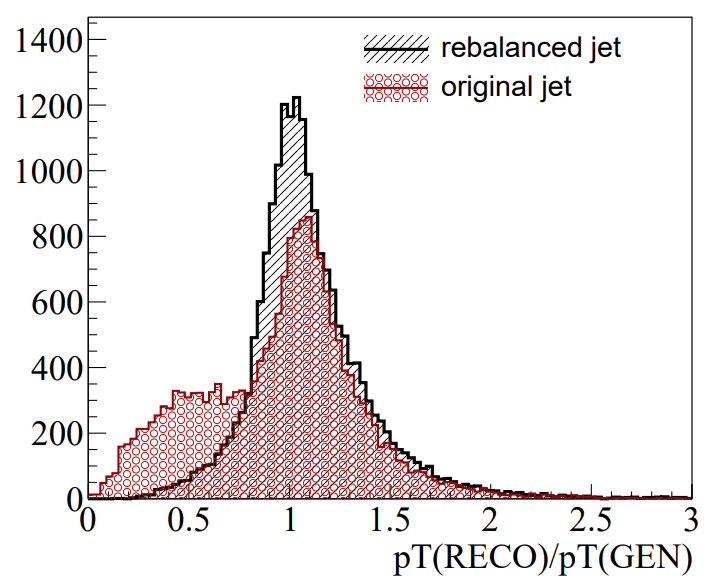
\includegraphics[width=0.7\linewidth]{Figures/RebalancedJetRes}
	\caption[Jet energy response for leading jets in QCD MC before and after rebalancing.]{Energy response for the leading jet in QCD MC events with $E_T^{miss}>120$ GeV before and after being rebalanced. The original jet collection is shown shaded in red while the rebalanced collection is shaded in black. The jet energy response is defined as the ratio of the reconstructed jet $p_T$ and the generator-level jet $p_T$ as described in Section \ref{section:jetalgorithm}.  Rebalancing improves the jet energy resolution and recovers some of the energy that was lost in original reconstruction of the jet.}
	\label{fig:rebalancedjetres}
\end{figure}

In the next step, the seed events obtained through rebalancing are smeared in order to simulate the expected detector-level measurement of each jet.  The smearing is done by scaling the $p_T$ of each jet by a random factor sampled from the full pre-rebalanced jet response distribution described in Section \ref{section:jetalgorithm}.  The smear step was performed 50 times on each seed event in order to probe more of the response distribution and improve prediction stability by decreasing the effect of statistical fluctuations.

The result of this process is that we are able to take events from real data, rebalance them to closer to truth-level, and then use those rebalanced events as seeds to generate multiple detector-level events.  This method has been proven effective in all-hadronic final states, but in this case it is being used in the presence of two photons also in the final state.  As the photon $p_T$ values in the seed events are not smeared like the jets to create these new detector-level events, there is a danger that the photon $p_T$ spectrum could be distorted.  This was checked using simulated di-photon events from QCD MC requiring two loose ID photons and Hard $E_T^{miss}>120$ GeV.  The results in Figures \ref{fig:randspho1closure} and \ref{fig:randspho2closure} show that there is no significant distortion of either the leading or next-to-leading photon $p_T$ spectra.

%\begin{figure}[h]
%	\centering
%	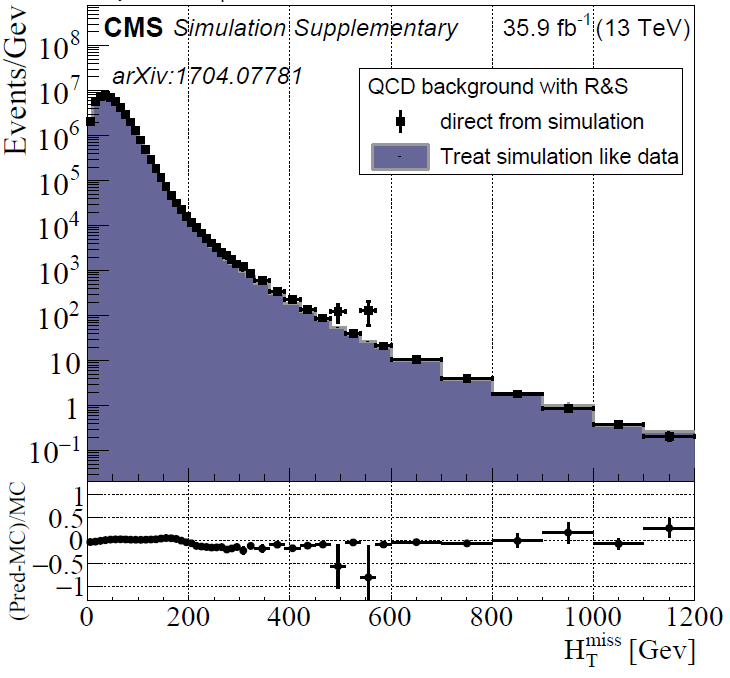
\includegraphics[width=0.9\linewidth]{Figures/RandSclosure}
%	\caption[Closure test for RandS]{RandS closure test.}
%	\label{fig:randsclosure}
%\end{figure}
\begin{figure}[h]
	\centering
	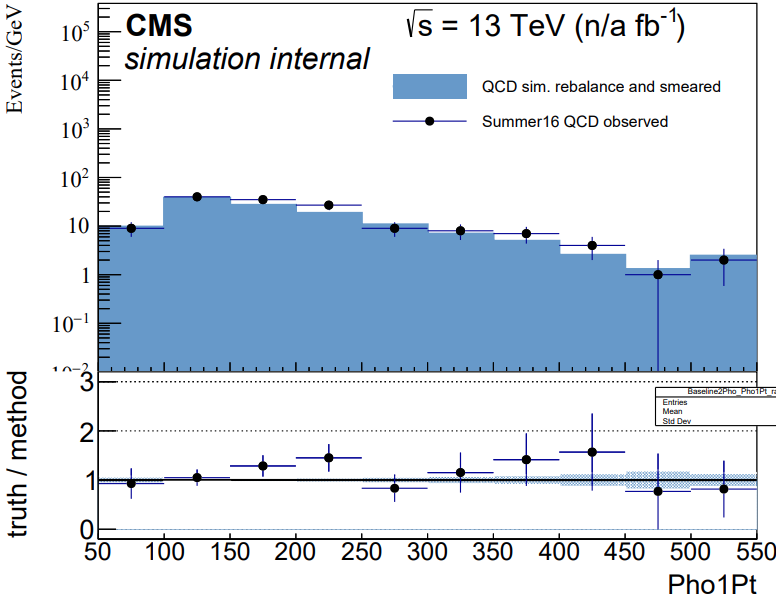
\includegraphics[width=0.9\linewidth]{Figures/RandS_Pho1_closure}
	\caption[Leading photon $p_T$ distrubutions for di-photon QCD MC events before and after Rebalance and Smear implimentation.]{This shows a comparison of the $p_t$ distribution for the leading photons in di-photon QCD MC events before and after being Ralanced and Smeared. These events were requireed to have two loose ID photons and Hard $E_T^{miss}>120$ GeV. The data points are taken directly from the QCD simulation while the blue shaded area shows the distribution after application of Rebalance and Smear. We see here that the Rebalance and Smear method causes no significant distortions to the leading photon $p_T$ spectrum in di-photon events.}
	\label{fig:randspho1closure}
\end{figure}
\begin{figure}[h]
	\centering
	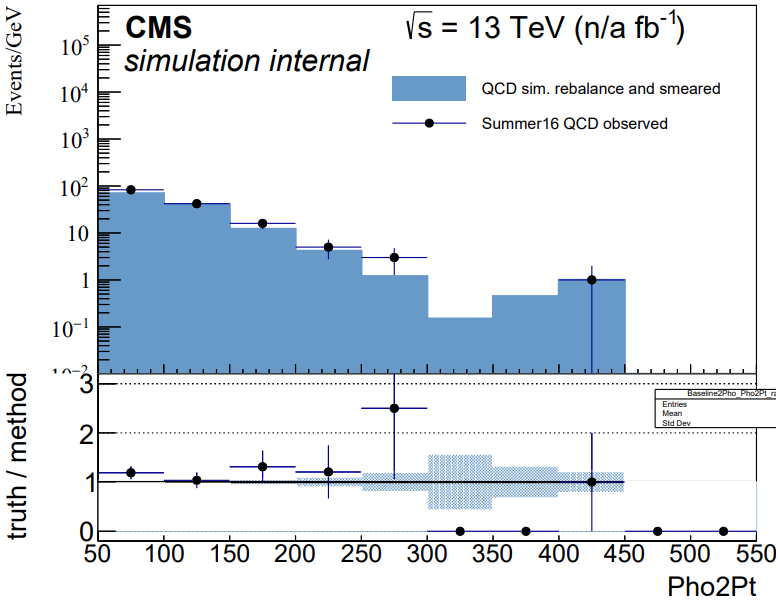
\includegraphics[width=0.9\linewidth]{Figures/RandS_Pho2_closure}
	\caption[Next-to-leading photon $p_T$ distrubutions for di-photon QCD MC events before and after Rebalance and Smear implimentation.]{This shows a comparison of the $p_t$ distribution for the next-to-leading photons in di-photon QCD MC events before and after being Ralanced and Smeared. These events were requireed to have two loose ID photons and Hard $E_T^{miss}>120$ GeV. The data points are taken directly from the QCD simulation while the blue shaded area shows the distribution after application of Rebalance and Smear. We see here that the Rebalance and Smear method causes no significant distortions to the next-to-leading photon $p_T$ spectrum in di-photon events.}
	\label{fig:randspho2closure}
\end{figure}

\label{section:RandS}
\subsubsection{Multivariate discriminant}
A boosted decision tree (BDT) was used to develop a discriminating variable for identifying events with real $E^{miss}_T$.  A decision tree is a classifier with a binary tree structure that recursively partitions data or samples into classifications of either signal or background.  Figure \ref{fig:decisiontree} shows an example schematic of a single decision tree.  Each splitting of the data takes place at a \textit{node}.  Each node uses a single input variable to make a decision regarding classification.  This process begins at a \textit{root} node and continues until the final node in the tree is reached, which is referred to as a \textit{leaf} node.  The number of layers of nodes is what we call the \textit{depth} of a tree.  \textit{Training} is the process of building or growing a tree.  The training process begins by setting an initial splitting criteria at a root node.  The root node splits the training data, which consists a set of background samples and a set of signal samples, into two subsets which each go to different node where this same process is repeated until the entire tree is built.  The splitting criteria at each node is determined by finding which variable and cut value on said variable results in the best separation between signal and background.  The amount of separation is quantified by a separation index known as the Gini Index, which is defined by $p(1-p)$ where is $p$ is the purity of the resulting subsets.  Once the entire tree is built, the leaf nodes are identified as either signal or background depending on whether the majority of the events they contain are from the signal or background training samples.
\begin{figure}[h]
	\centering
	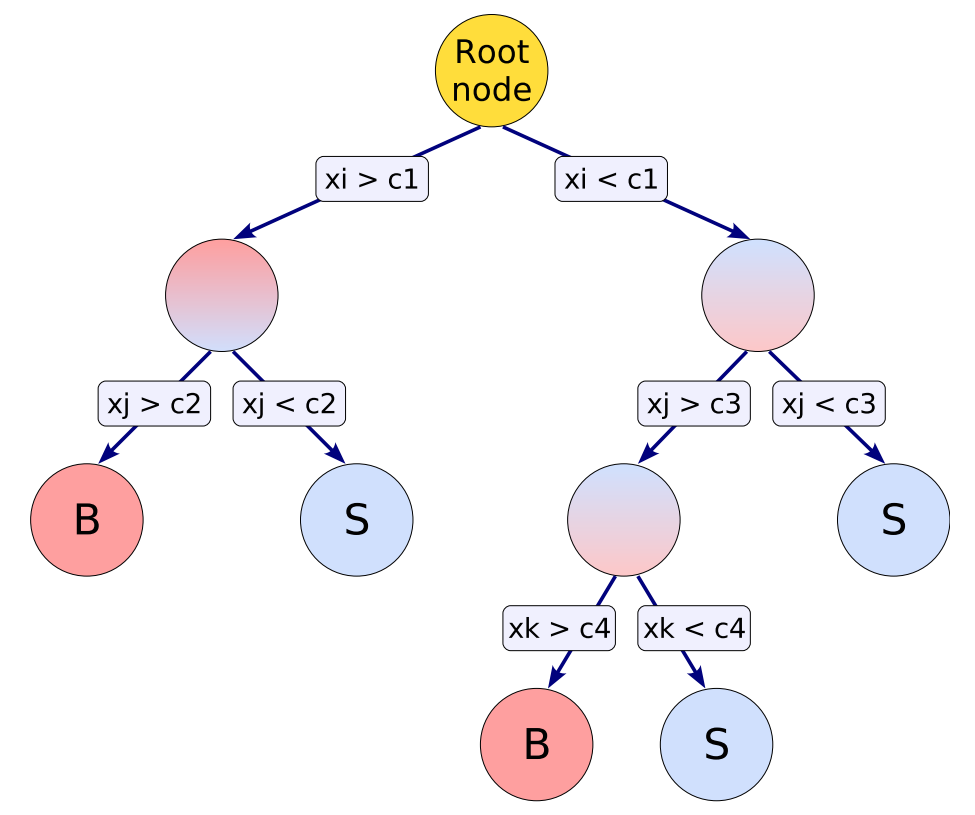
\includegraphics[width=1.0\linewidth]{Figures/decisiontree}
	\caption[Schematic view of a decision tree.]{This is a schematic view of a decision tree. Reprint from \cite{Hocker:2007ht}}
	\label{fig:decisiontree}
\end{figure}

Extending this process to many trees, which we call a \textit{forest}, allows us to enhance the classification performance by applying a  \textit{boosting} algorithm.  For this analysis the AdaBoost (adaptive boost) algorithm was used.  The AdaBoost algorthm gives added weight (boost weight) to events in the training sample that misidentified as either signal or background and then uses these reweighted events as the training sample for growing the next tree.  The boost weight is given as
\begin{equation}
	\alpha = \frac{1-\epsilon}{\epsilon}
\end{equation}
where $\epsilon$ is the misclassification rate of the previous tree.  The same $\alpha$ is applied to every event that was misclassified in the training sample. The boosted classification, or BDT score, is then given by
\begin{equation}
	BDT_{score}(x) = \frac{1}{N_{trees}}\cdot\sum_{i}^{N_{trees}}\ln(\alpha_i)\cdot h_i(x)
\end{equation}
where $x$ is the set of input variables, and $h(x)$ = 1 if the event falls into a signal leaf and -1 if it is in a background leaf.  The result is a $BDT_{score}$ that ranges between -1 (background-like) and +1 (signal-like).

Training and testing of the BDT was performed in ROOT using the Toolkit for MultiVariate Analysis (TMVA).  The signal samples used for both training and testing are comprised of a combination of different mass points from the T5Wg and T6Wg MC samples.  The mass points used were chosen to represent a wide range of mass differences between gluino/squark and neutralino masses.  This was done by using the bands of gluino/squark masses shown in Figure \ref{fig:massbands}.   
\begin{figure}[h]
	\centering
	\subfloat[Cross-section upper limits with 95\% confidence level for gluino pair production][Cross-section upper limits for gluino pair production]{
		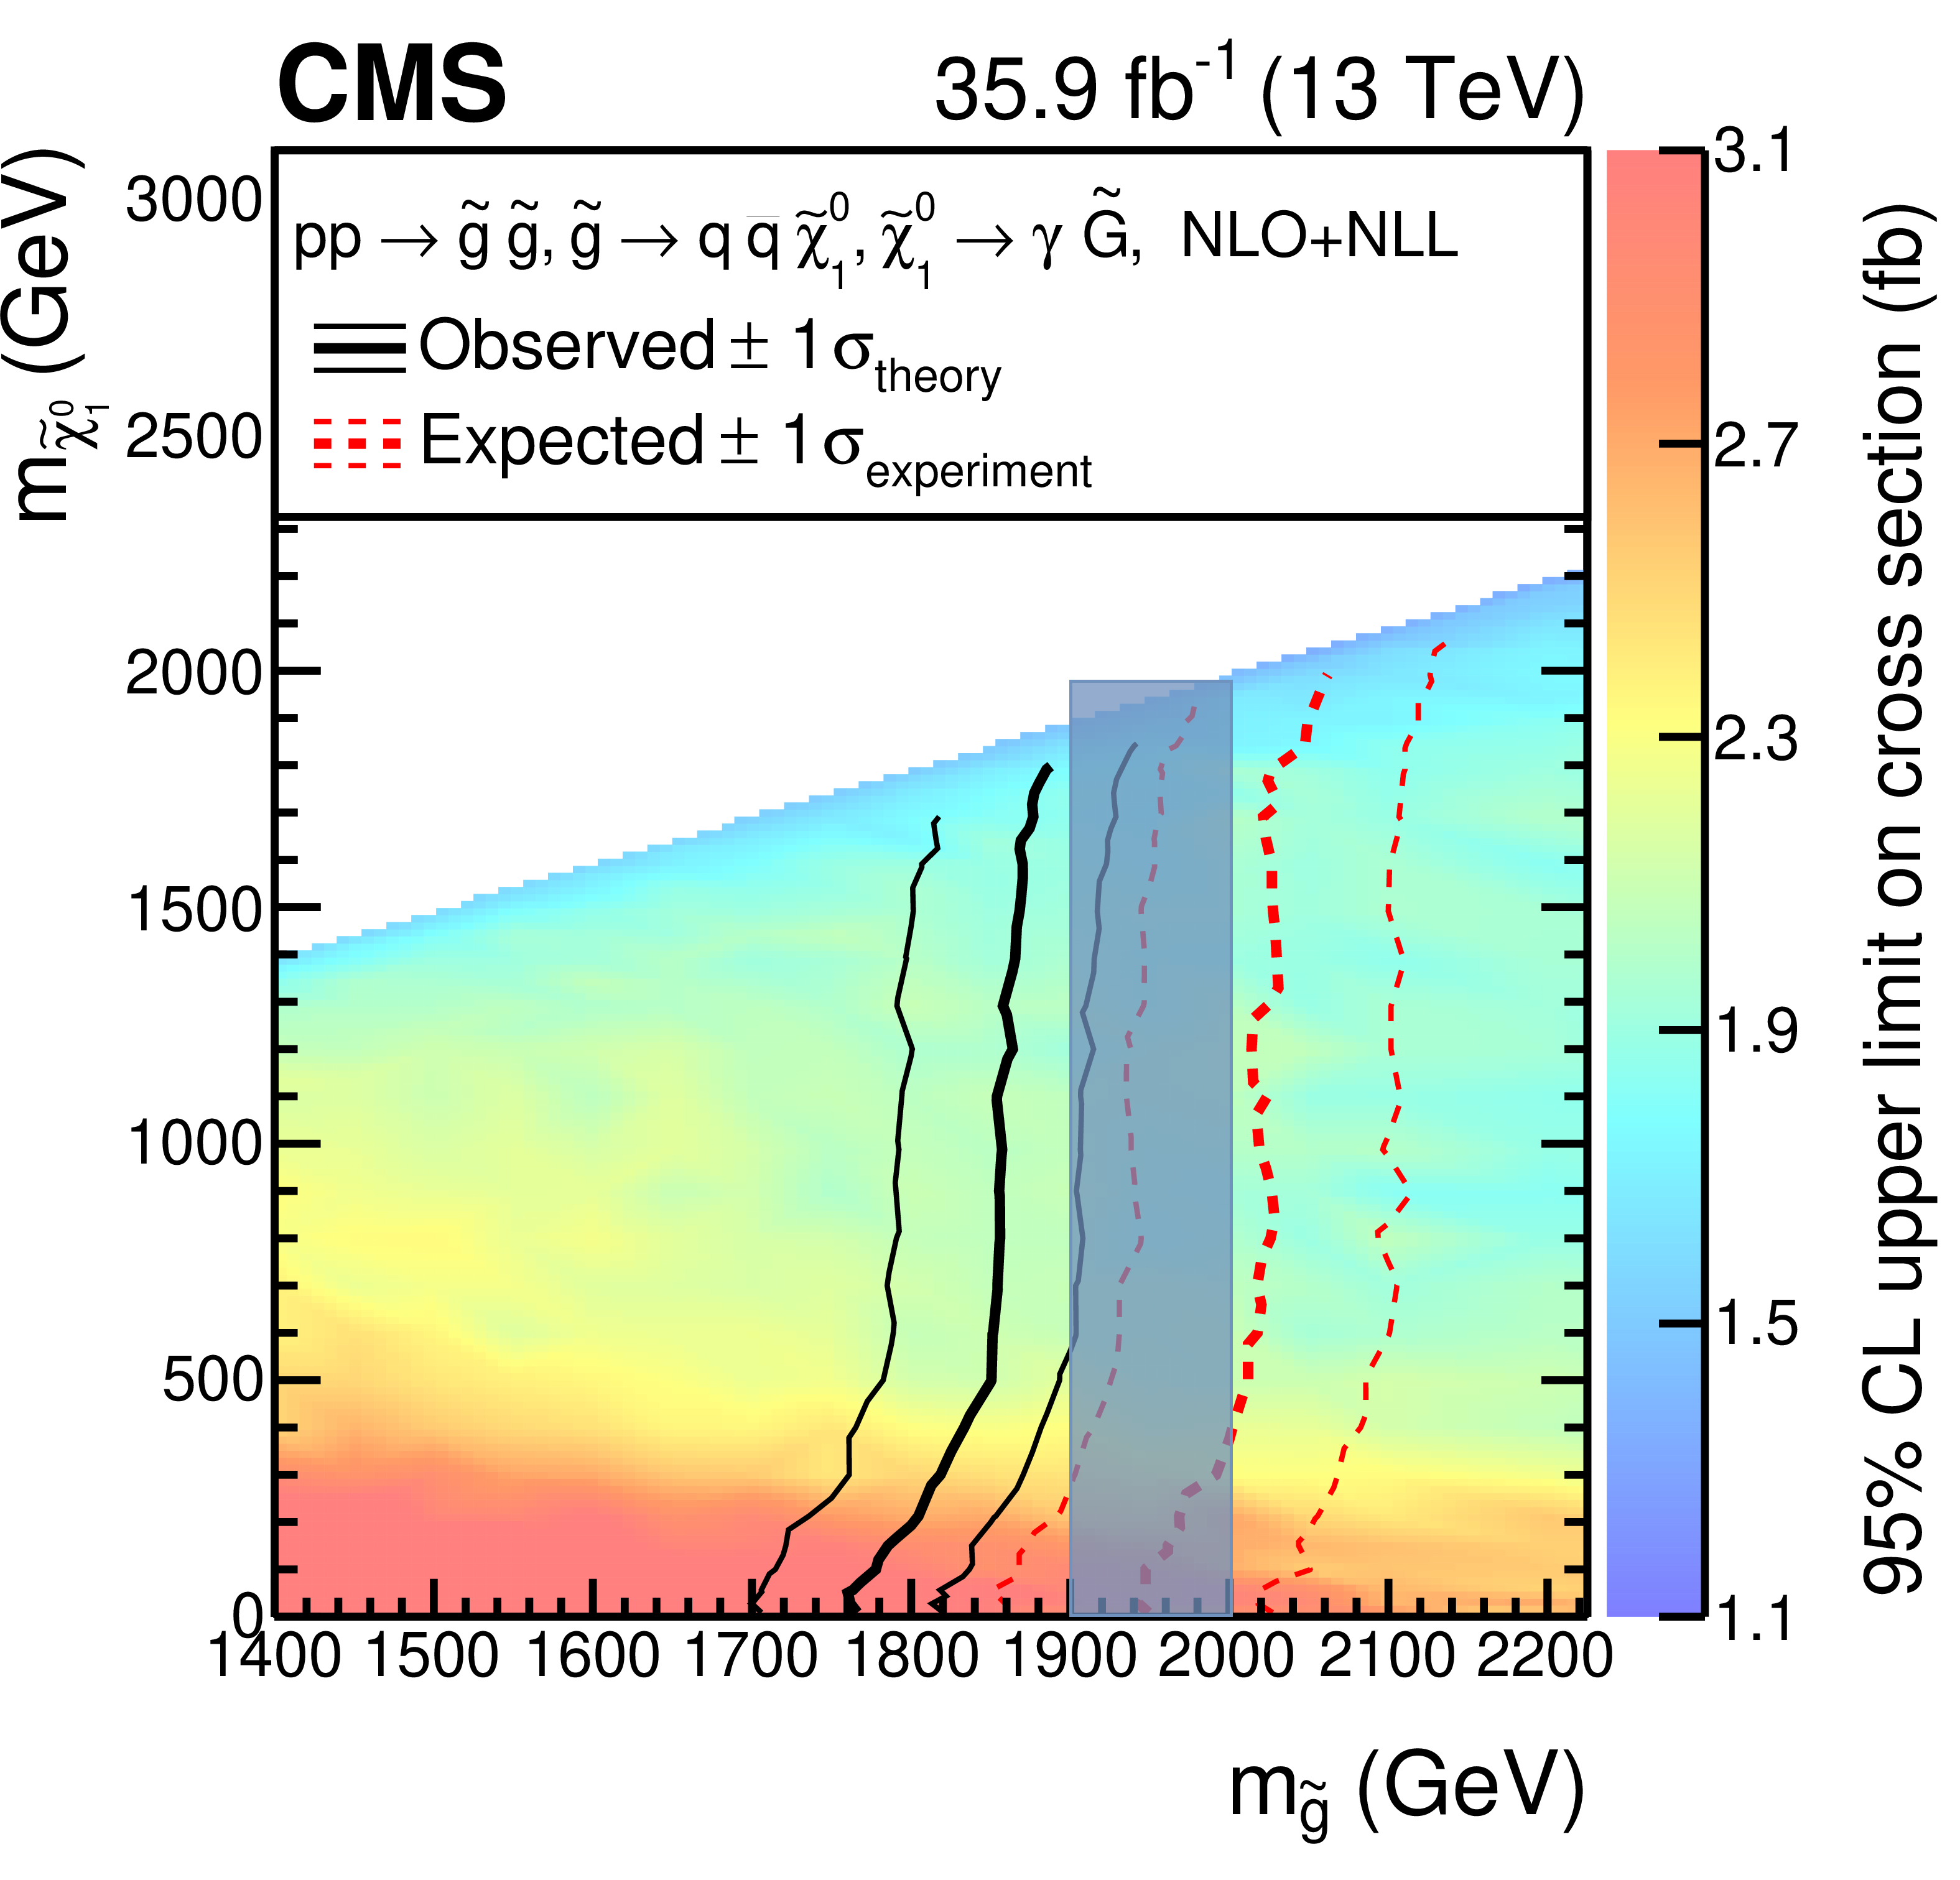
\includegraphics[width=0.7\textwidth]{Figures/OldLimits_gluino_withmassband}
		\label{fig:gluinomassband}}
	\qquad
	\subfloat[Cross-section upper limits with 95\% confidence level for squark pair production][Cross-section upper limits for squark pair production]{
		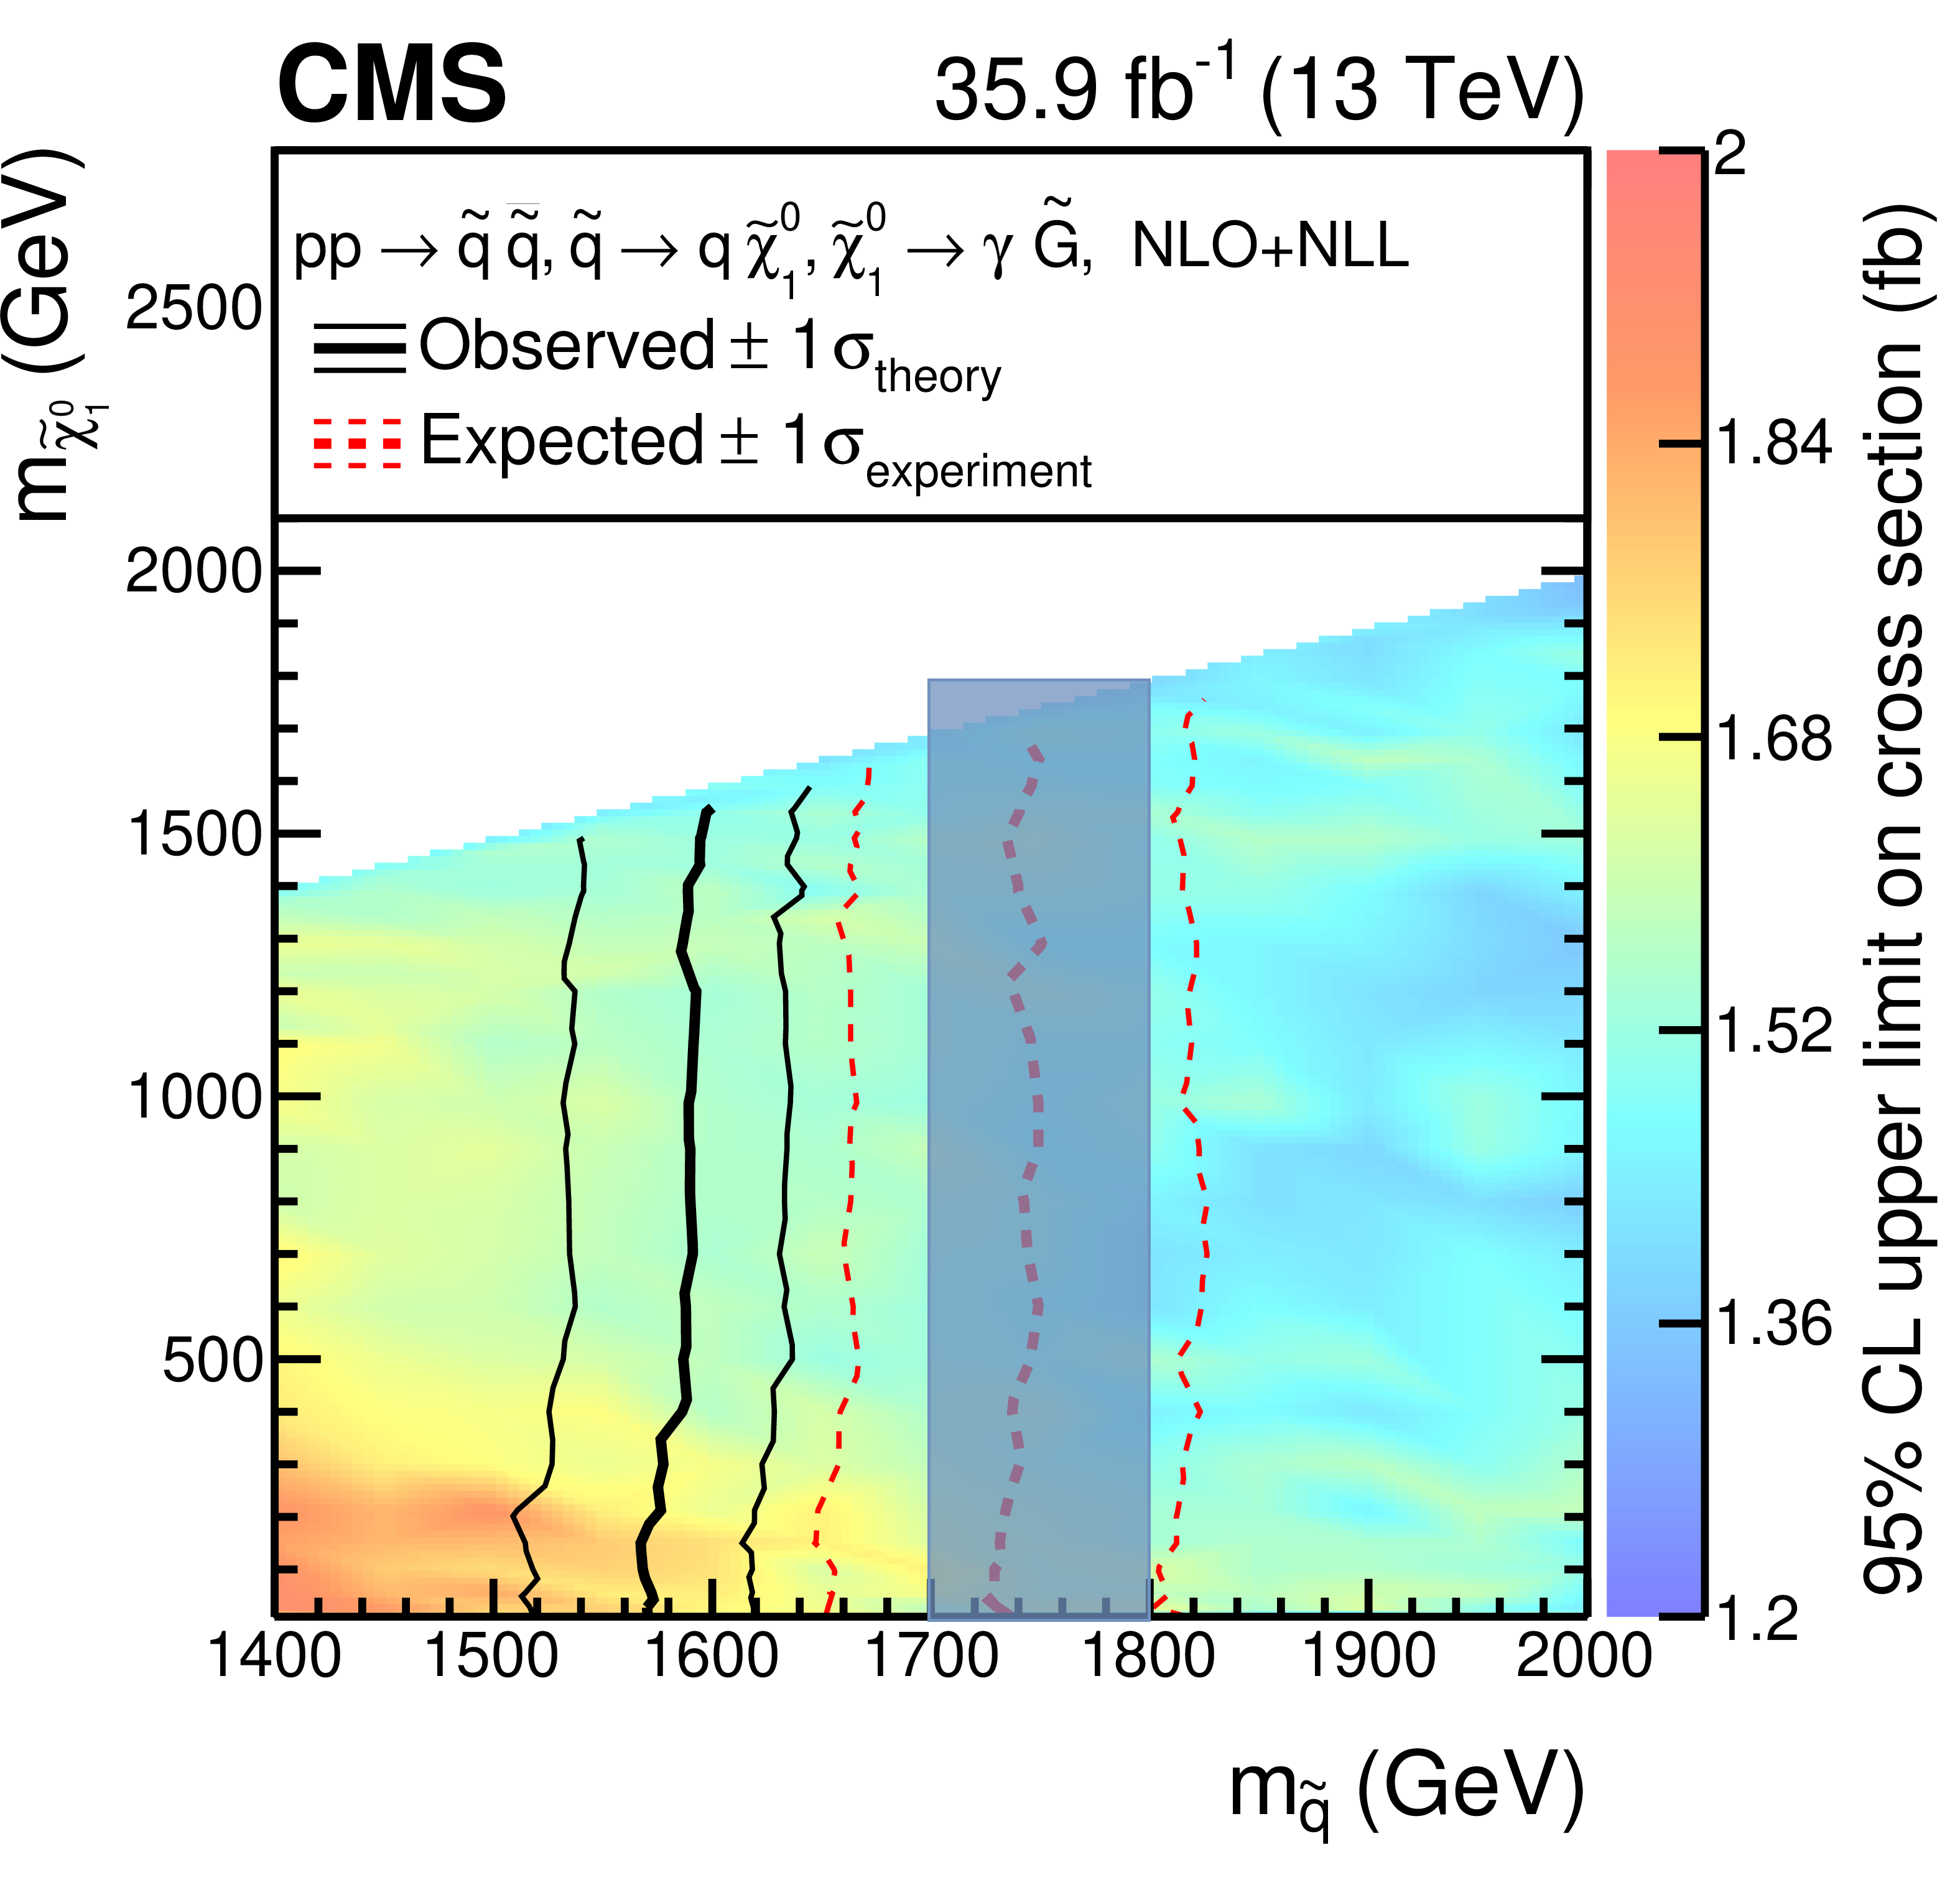
\includegraphics[width=0.7\textwidth]{Figures/OldLimit_squark_withmassband}
		\label{fig:squarkmassband}}
	\caption{The 95\% confidence level upper limits on the pair production cross sections for gluinos (\ref{fig:gluinomassband})and squarks (\ref{fig:squarkmassband})as a function of gluino/squark and neutralino masses as reported in \cite{CMS:OldSUSYpaper}.  The shaded vertical bands show the mass bands used in the BDT training.}
	\label{fig:massbands}
\end{figure}
In order to minimize any bias in the BDT response to  model-dependent parameters like the difference between gluino/squark and neutralino masses, the training events used from each mass point were weighted by a factor of one over the number events generated for that particular model.  This ensures that each mass point in the mass band is equally represented in the training sample for the BDT.  The location of the mass bands were chosen to be near the edge of the exclusion region to target the phase space not yet ruled out by previous analyses.  The background samples use for training and testing of the BDT were GJets MC samples that had been Rebalanced and Smeared to increase statistics. These simulate Standard Model processes resulting in final states containing jets and at least one photon which is the source of the fake $E^{miss}_T$ background.  The full list of MC samples used in the BDT training can be seen in Table \ref{table:TrainingSamples}.  As mentioned in Section \ref{section:pixelupgrade}, there was a substantial upgrade to the pixel detector in between 2016 and 2017 which separates Run 2 into Phase 0 (2016) and Phase 1 (2017 and 2018).  In order to remove any effects on the BDT due to different detector response before and after the upgrade, a separate BDT was trained and applied for each of these two phases.  For events from these samples to be included in the training or testing of the BDT, they were required to have
\begin{itemize}
	\item At least two photons without associated pixel seeds as described in Section \ref{section:photondefinition}.
	\item At least one of those photons is in the EB ($|\eta|<1.44$)
	\item Both photons within the range of tracker acceptance ($|\eta|<2.4$)
	\item At least two jets as described in Section \ref{section:jetdefinition}.
	\item Hard $E^{miss}_T>130$ GeV
\end{itemize}

\begin{table}[h]
	\centering
	\caption{List of MC samples used for training and testing BDT}
	\begin{tabular}{|c|}
		\hline
		\textbf{Signal Samples} \\  
		\hline
		SMS-T5Wg\_TuneCUETP8M1\_13TeV-madgraphMLM-pythia8\\
		\hline
		SMS-T6Wg\_TuneCUETP8M1\_13TeV-madgraphMLM-pythia8\\
		\hline
		\textbf{Background Sample} \\ 
		\hline
		GJets\_DR-0p4\_HT-100To200\_TuneCUETP8M1\_13TeV-madgraphMLM-pythia8 \\
		\hline
		GJets\_DR-0p4\_HT-200To400\_TuneCUETP8M1\_13TeV-madgraphMLM-pythia8 \\
		\hline
		GJets\_DR-0p4\_HT-400To600\_TuneCUETP8M1\_13TeV-madgraphMLM-pythia8 \\
		\hline
		GJets\_DR-0p4\_HT-600ToInf\_TuneCUETP8M1\_13TeV-madgraphMLM-pythia8 \\
		\hline
	\end{tabular}
	\label{table:TrainingSamples}
\end{table}

 The input variables used by the BDT are listed below.  All energy and momentum variables were normalized to the scalar sum of all of the $p_T$ in the event $S_T = \sum_{\gamma,jets} |\vec{p}_{T_i}|$ in order to encourage the BDT to focus more on how the energy and momentum was distributed in an event rather than simply the scale of the energy or momentum.  Distributions of the input variables for both signal and background are shown in Figure \ref{fig:bdtvar1}, \ref{fig:bdtvar2}, and \ref{fig:bdtvar3}.

\begin{itemize}
	\item $S_{T_{jets}} = \sum_{jets}|\vec{p}_T|$
	\item $p_{T_{jets}} = \sum_{jets}\vec{p}_T$
	\item $p_{T_{\gamma \gamma}} = \vec{p}_{T_{\gamma_1}} + \vec{p}_{T_{\gamma_2}}$
	\item $Hard E_T^{miss} = |-\sum_{i}\vec{p_{Ti}}\cdot \Theta(30 -p_{Ti})|$
	\item $\Delta \Phi_{\gamma \gamma} = \Delta \Phi (\vec{p}_{T_{\gamma_1}}, \vec{p}_{T_{\gamma_2}})$
	\item $\Delta \Phi_{min} = min[\Delta \Phi (\vec{p}_{T_{HardE_T^{miss}}}, \vec{p}_{T_{jet_i}})]$
	\item $\Delta \Phi_{1} = \Delta \Phi (\vec{p}_{T_{HardE_T^{miss}}}, \vec{p}_{T_{jet_1}})$
	\item $\Delta \Phi_{2} = \Delta \Phi (\vec{p}_{T_{HardE_T^{miss}}}, \vec{p}_{T_{jet_2}})$
	\item $\Delta \Phi_{\gamma \gamma, HardE_T^{miss}} = \Delta \Phi (\vec{p}_{T_{HardE_T^{miss}}}, \vec{p}_{T_{\gamma \gamma}})$
	\item $\Delta R_{jet_n\gamma_m} = \Delta R(jet_n, \gamma_m) \text{ for } n=1,2 \text{ and } m=1,2$
\end{itemize}

\begin{figure}[h]
	\centering
	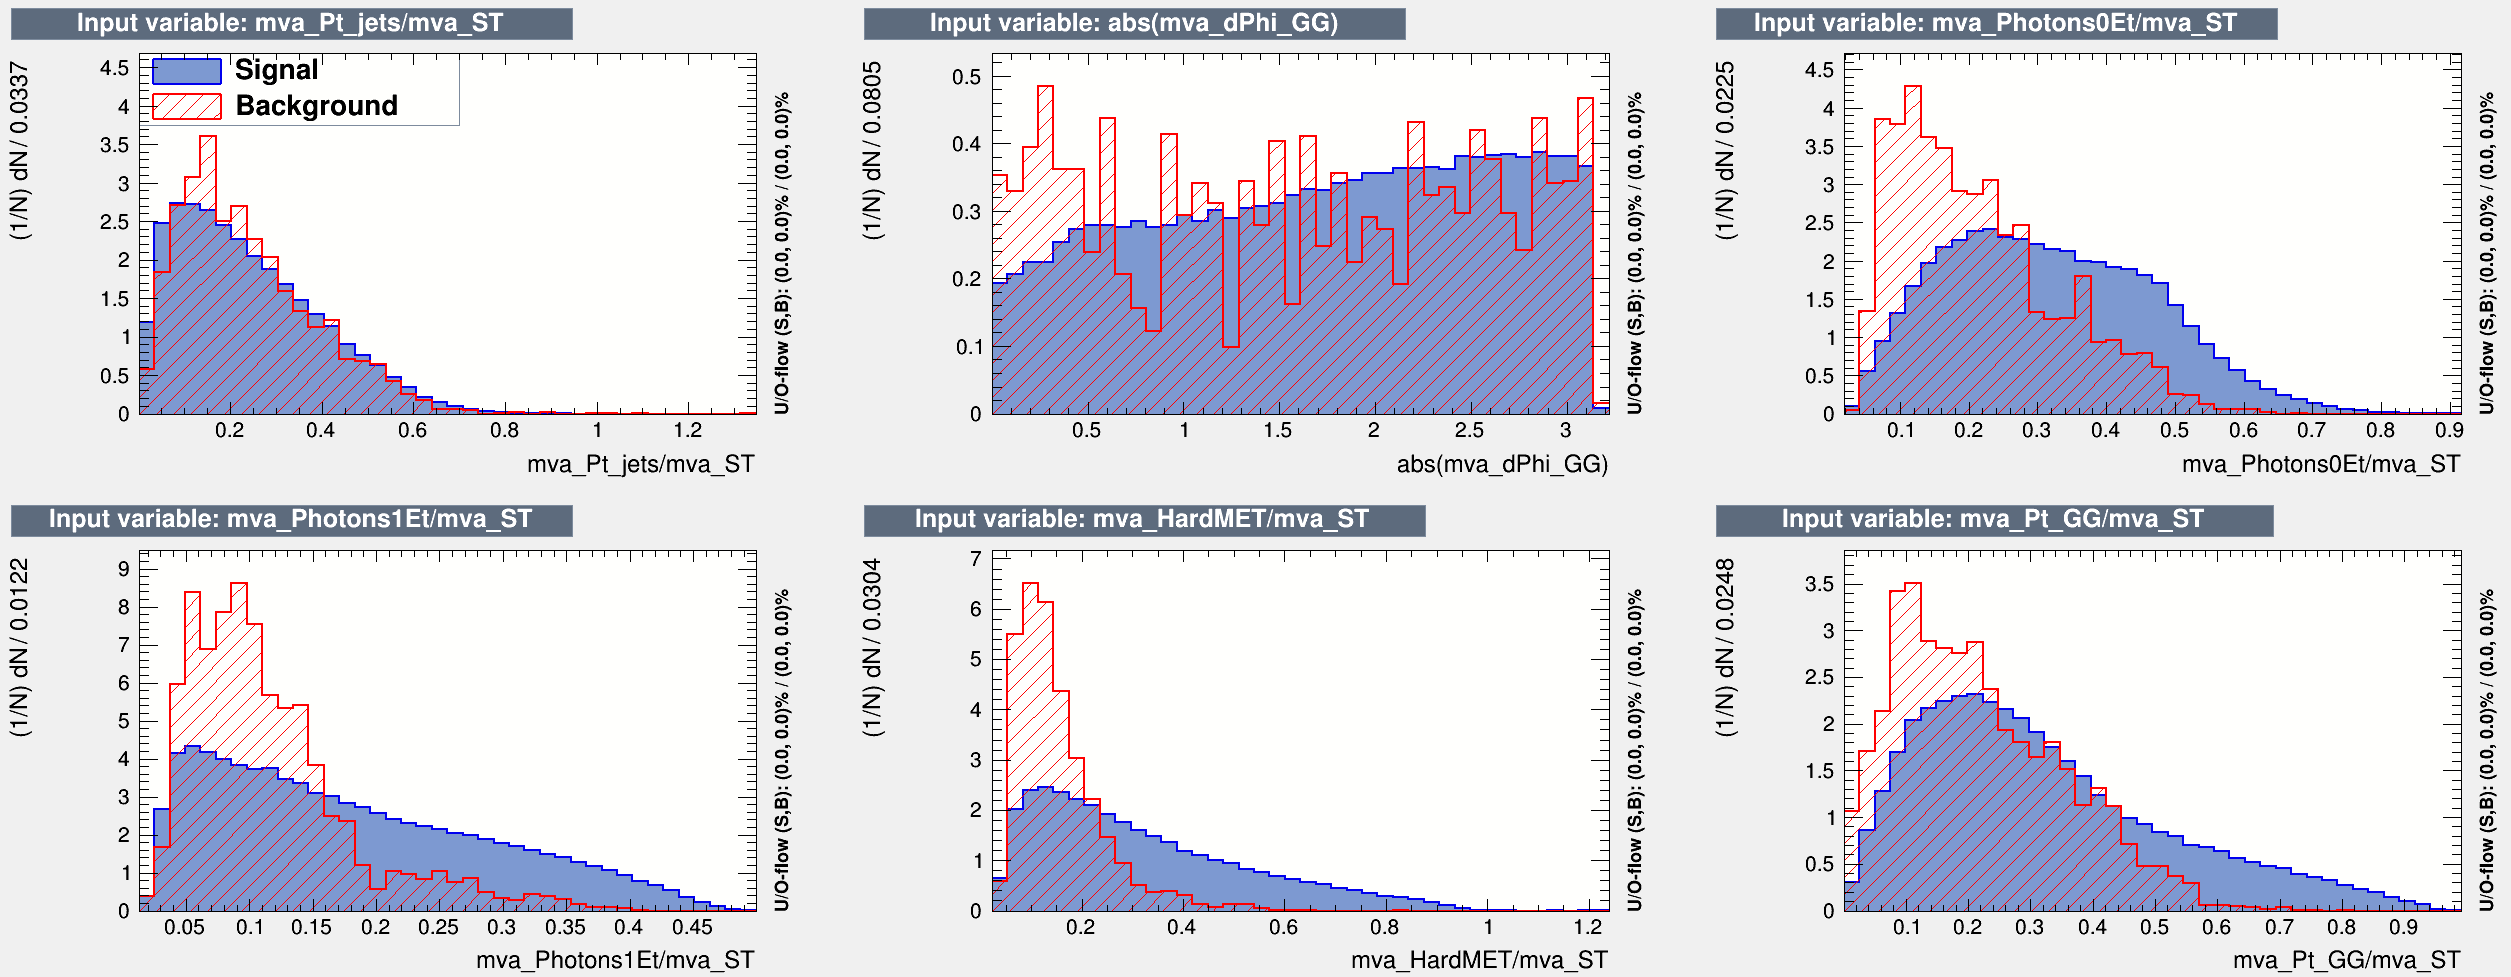
\includegraphics[width=1.7\linewidth, height=0.5\textheight, angle=90]{Figures/BDTvar1}
	\caption[BDT input variables 1]{Signal and background input variable distributions for the BDT.  The red distribution represents the background while the blue is signal.}
	\label{fig:bdtvar1}
\end{figure}

\begin{figure}[h]
	\centering
	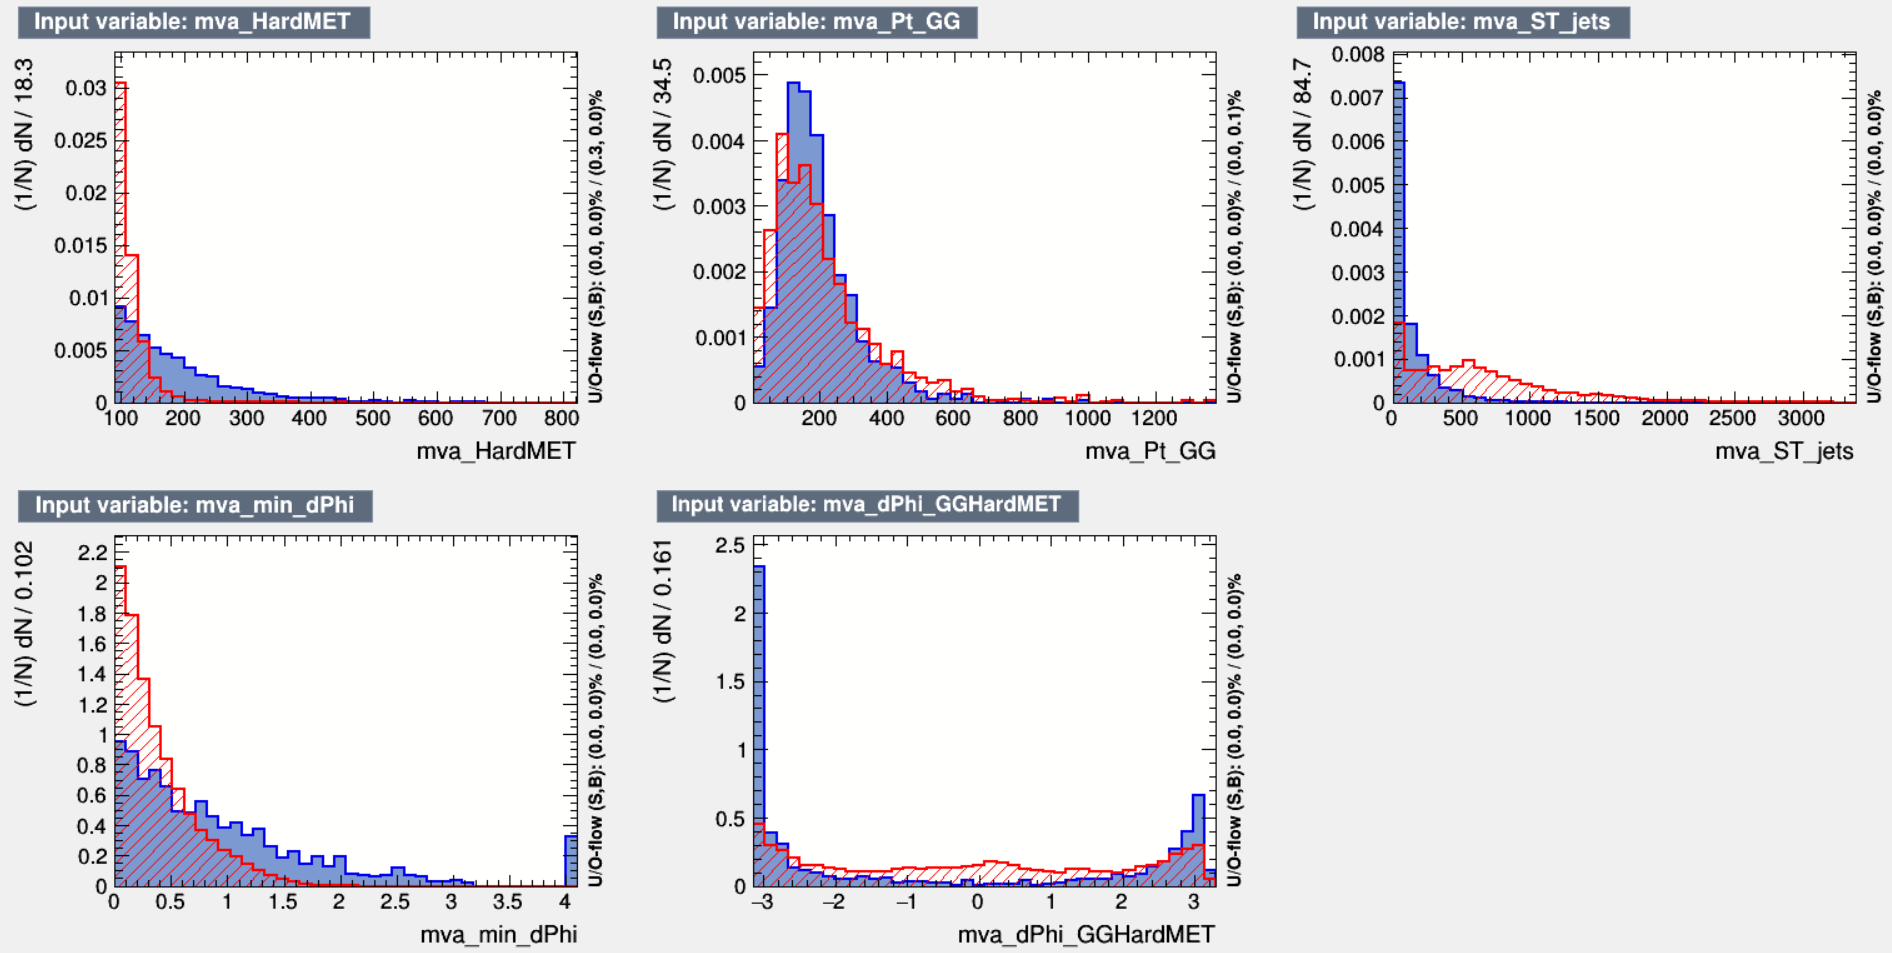
\includegraphics[width=1.7\linewidth, height=0.5\textheight, angle=90]{Figures/BDTvar2}
	\caption[BDT input variables 2]{More signal and background input variable distributions for the BDT.  The red distribution represents the background while the blue is signal.}
	\label{fig:bdtvar2}
\end{figure}

\begin{figure}[h]
	\centering
	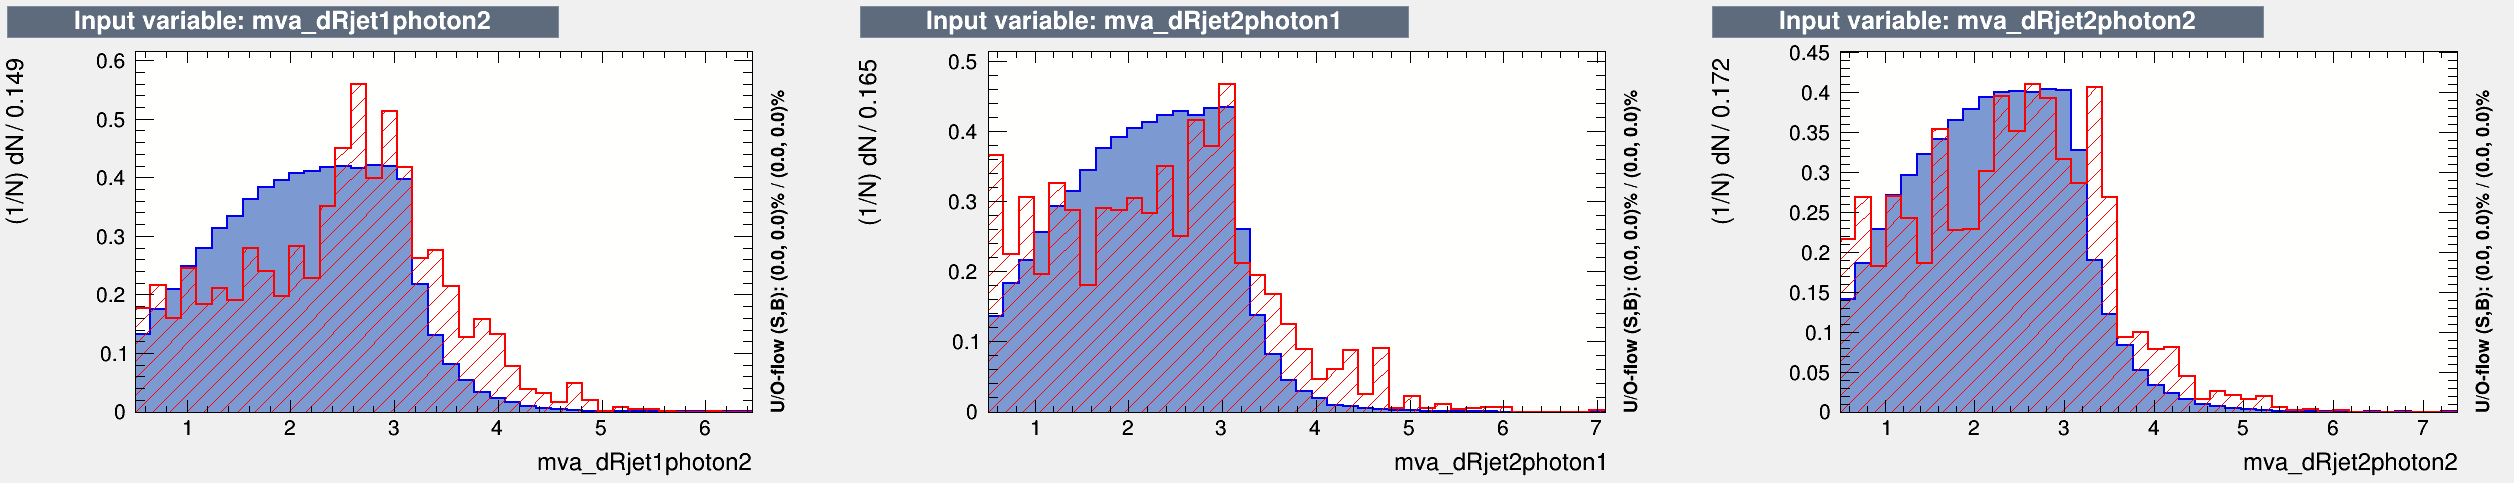
\includegraphics[width=1.7\linewidth, height=0.3\textheight, angle=90]{Figures/BDTvar3}
	\caption[BDT input variables 3]{More signal and background input variable distributions for the BDT.  The red distribution represents the background while the blue is signal.}
	\label{fig:bdtvar3}
\end{figure}

Events in both the signal and background samples are randomly split into either a test or training categories.  A substantial difference between the test and training distributions of the BDT response implies that the BDT is not drawing reliable conclusions as to whether an event is signal-like or background-like.  A grid search over different combinations of hyperparameters (the maximum depth of a tree and the number of trees) was performed to maximize separation between the signal and background BDT response distributions while maintaining good agreement between the training and test samples.  Using 200 trees with a maximum depth of 4 was found to be the optimal choice as increasing either or both of those parameters resulted in over-training with minimal gains in separation of signal and background. The comparison of BDT scores between signal and background events is shown in Figures \ref{fig:phase0bdtresponse} and \ref{fig:phase1bdtresponse} for the Phase 0 and Phase 1 BDTs respectively.  Comparisons of training and test samples for Phase 0 are shown in Figures \ref{fig:phase0bdtbkgotcheck} (background) and \ref{fig:phase0bdtsignalotcheck} (signal).  The comparisons for Phase 1 are shown in Figures \ref{fig:phase1bdtbkgotcheck} (background) and \ref{fig:phase1bdtsignalotcheck} (signal). The training and test samples comparisons don't show any significant deviations while there is good separation between signal and background BDT responses.

%\begin{figure}[h]
%	\centering
%	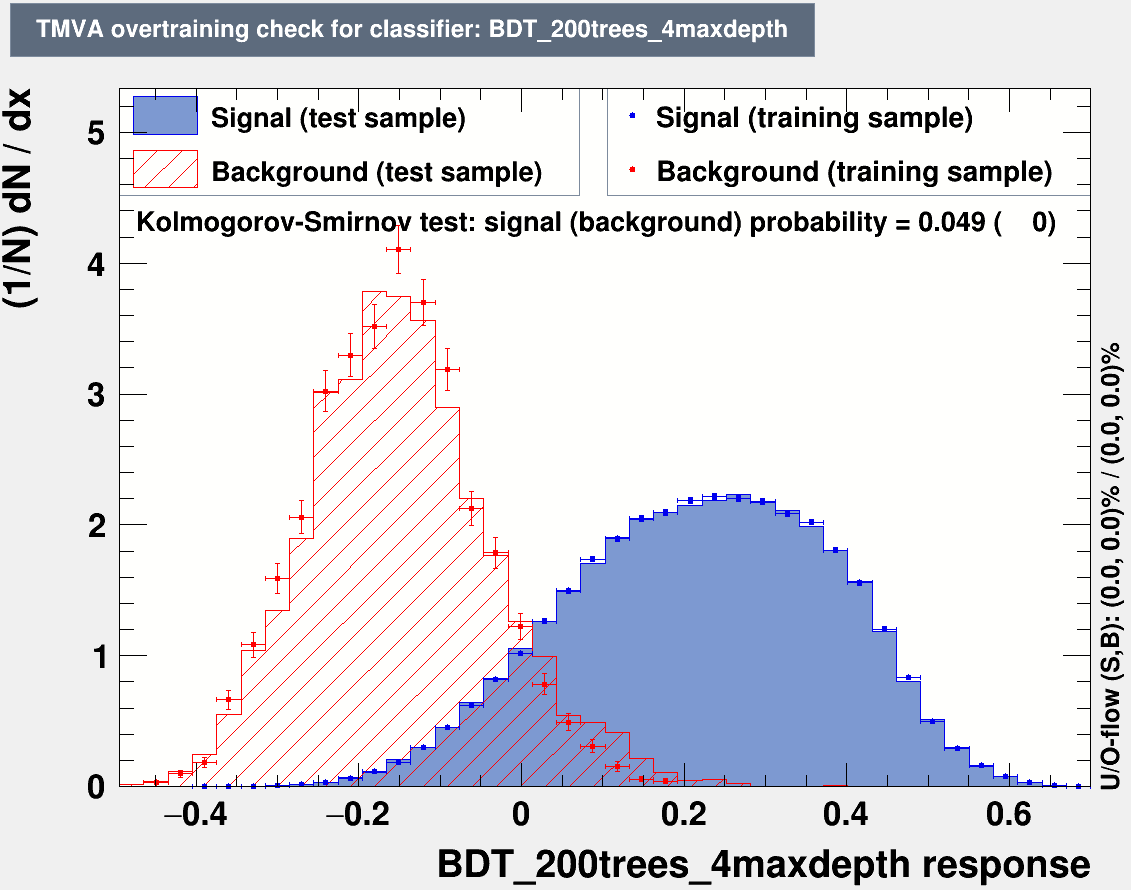
\includegraphics[width=1.0\linewidth]{Figures/BDT_response}
%	\caption[BDT training and testing results]{BDT score distributions for signal (blue) and background (red) events.  The shaded area shows the distribution of events in the test samples while t%he dots represent events in the training samples.}
%	\label{fig:bdtresponse}
%\end{figure}

\begin{figure}[h]
	\centering
	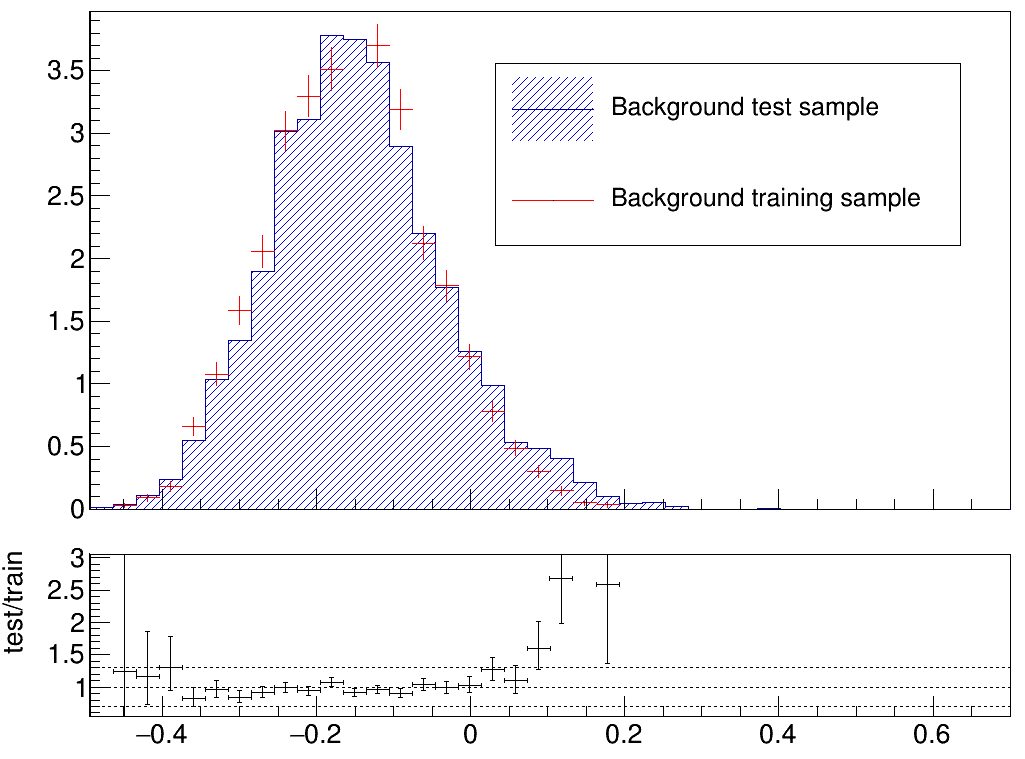
\includegraphics[width=0.9\linewidth]{Figures/Phase0BDT_bkgOTcheck}
	\caption[Overtraining check for background samples in Phase 0 BDT.]{Overtraining check for background samples in Phase 0 BDT.  The BDT score distributions for the training (red) and testing (blue) samples are plotted on the same graph.}
	\label{fig:phase0bdtbkgotcheck}
\end{figure}
\begin{figure}[h]
	\centering
	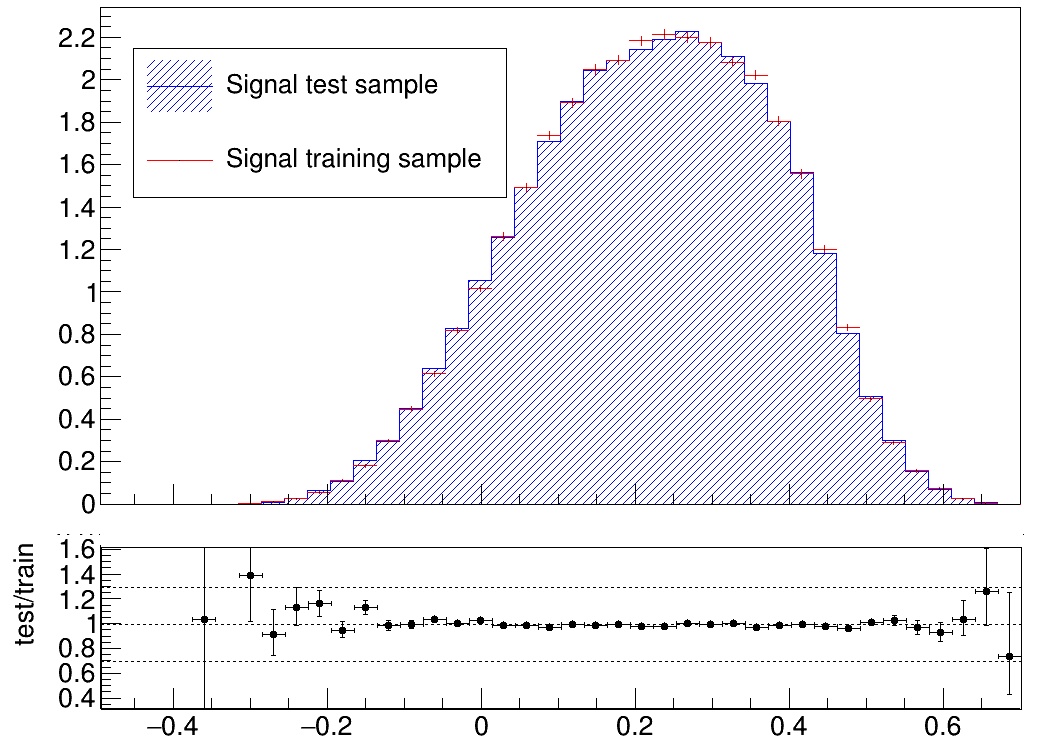
\includegraphics[width=0.9\linewidth]{Figures/Phase0BDT_signalOTcheck}
	\caption[Overtraining check for signal samples in Phase 0 BDT.]{Overtraining check for signal samples in Phase 0 BDT.  The BDT score distributions for the training (red) and testing (blue) samples are plotted on the same graph.}
	\label{fig:phase0bdtsignalotcheck}
\end{figure}
\begin{figure}[h]
	\centering
	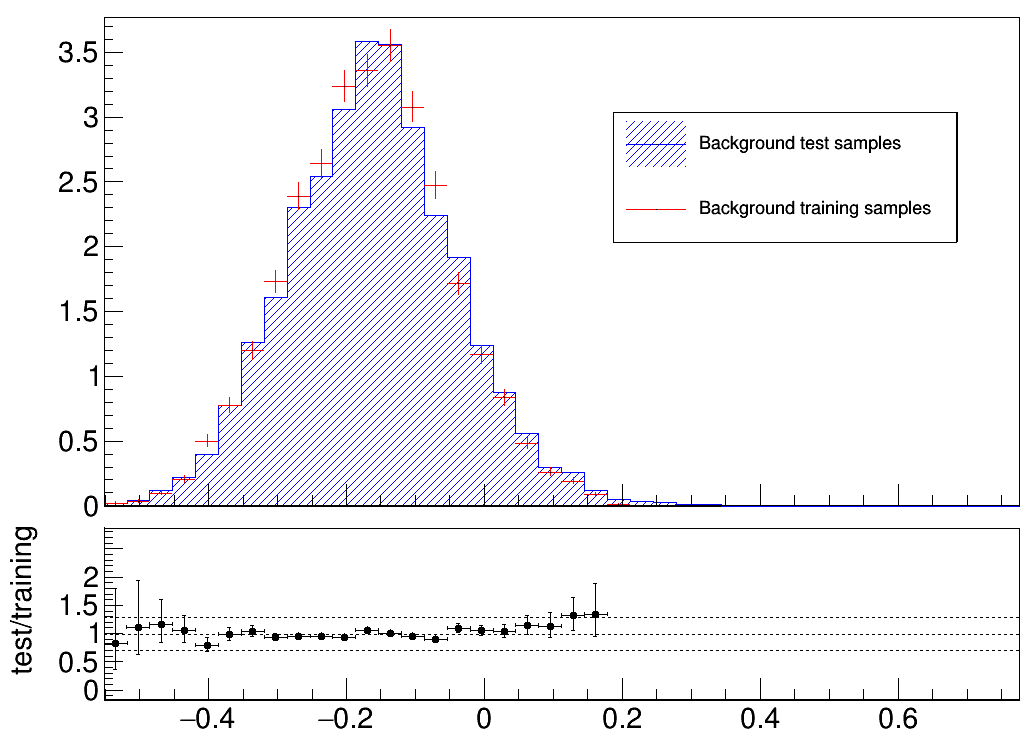
\includegraphics[width=0.9\linewidth]{Figures/Phase1BDT_bkgOTcheck}
	\caption[Overtraining check for background samples in Phase 1 BDT.]{Overtraining check for background samples in Phase 1 BDT.  The BDT score distributions for the training (red) and testing (blue) samples are plotted on the same graph.}
	\label{fig:phase1bdtbkgotcheck}
\end{figure}
\begin{figure}[h]
	\centering
	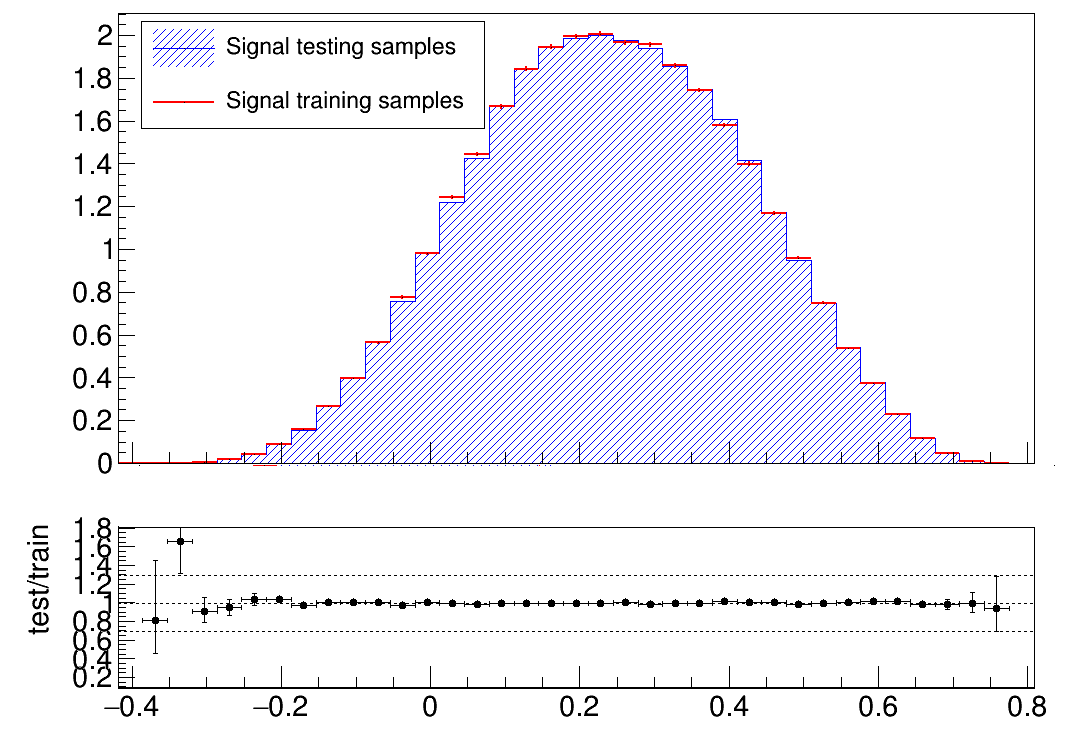
\includegraphics[width=0.9\linewidth]{Figures/Phase1BDT_signalOTcheck}
	\caption[Overtraining check for signal samples in Phase 1 BDT.]{Overtraining check for signal samples in Phase 1 BDT.  The BDT score distributions for the training (red) and testing (blue) samples are plotted on the same graph.}
	\label{fig:phase1bdtsignalotcheck}
\end{figure}
\begin{figure}[h]
	\centering
	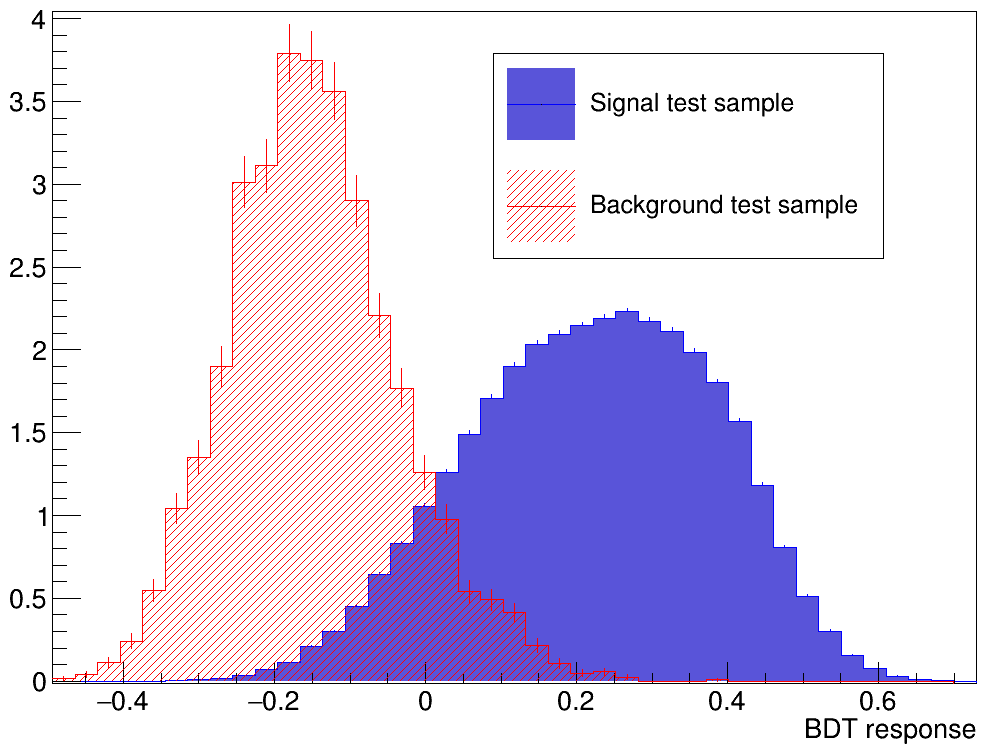
\includegraphics[width=0.9\linewidth]{Figures/Phase0BDTresponse}
	\caption[Phase 0 BDT response for signal and background]{Phase 0 BDT response for signal (blue) and background (red)}
	\label{fig:phase0bdtresponse}
\end{figure}
\begin{figure}[h]
	\centering
	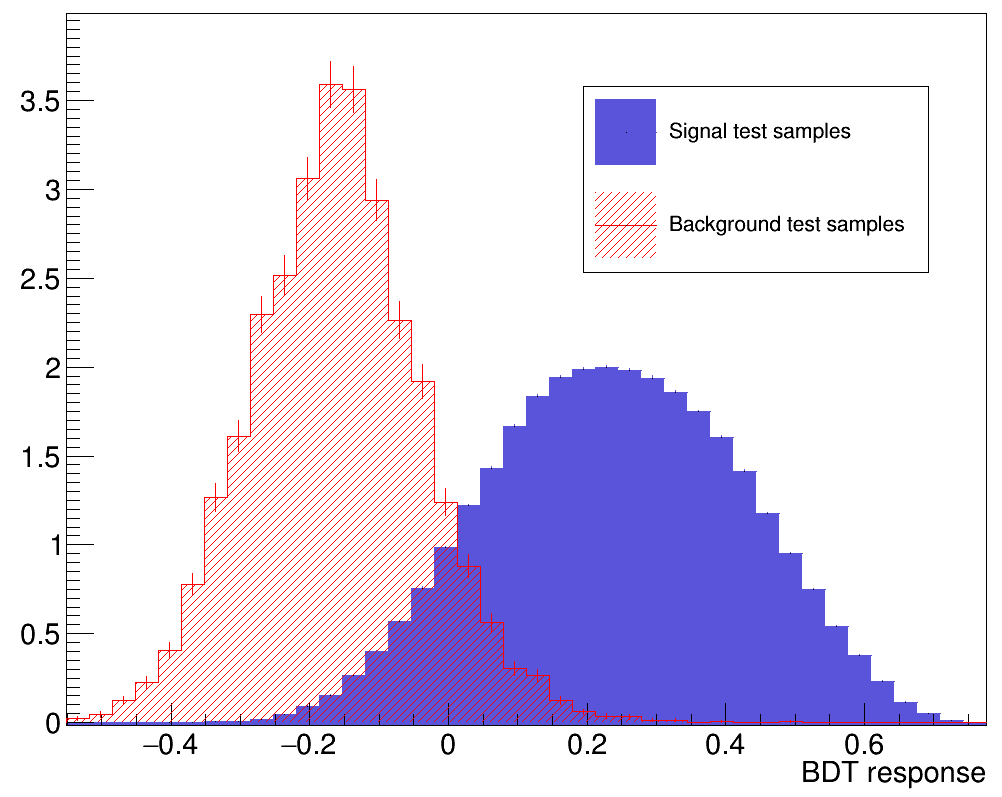
\includegraphics[width=0.9\linewidth]{Figures/Phase1BDTresponse}
	\caption[Phase 1 BDT response for signal and background]{Phase 1 BDT response for signal (blue) and background (red)}
	\label{fig:phase1bdtresponse}
\end{figure}


Using the BDT we created one control region (low BDT score) and two signal regions (medium and high BDT scores) by defining two BDT score thresholds.  The low threshold corresponds to the minimum BDT score with at least 90\% acceptance of every signal model or mass point in signal MC samples.  Figures \ref{fig:t5wgbdtcuts} and \ref{fig:t6wgbdtcuts} show the BDT cuts that resulted in 90\% acceptance at each mass point for the T5gg and T6gg models respectively.  In both models the value of this BDT cut is always greater than $-0.13$ so this was chosen as the value separating the low-BDT control region and the medium-BDT signal region.  The threshold for the high-BDT region is chosen such that 90\% of the fake $E^{miss}_T$ background from the GJets MC is excluded.  The BDT response for Rebalanced and Smeared events in this sample for each year is shown in Figures \ref{fig:bdtgjets}, \ref{fig:bdtgjets2017}, and \ref{fig:bdtgjets2018} where over 90\% of the events have a score less than $0.03$.  This puts the threshold for the high-BDT signal region at a BDT score of $0.03$.  With these three regions we have a very background-pure control region ($BDT \leq -0.13$) and two signal regions, one very pure in signal ($BDT\textgreater 0.03$) and one intermediate ($-0.13 \textless BDT \leq 0.03$), which combined have at least 90\% acceptance for all mass points.

\begin{figure}[h]
	\centering
	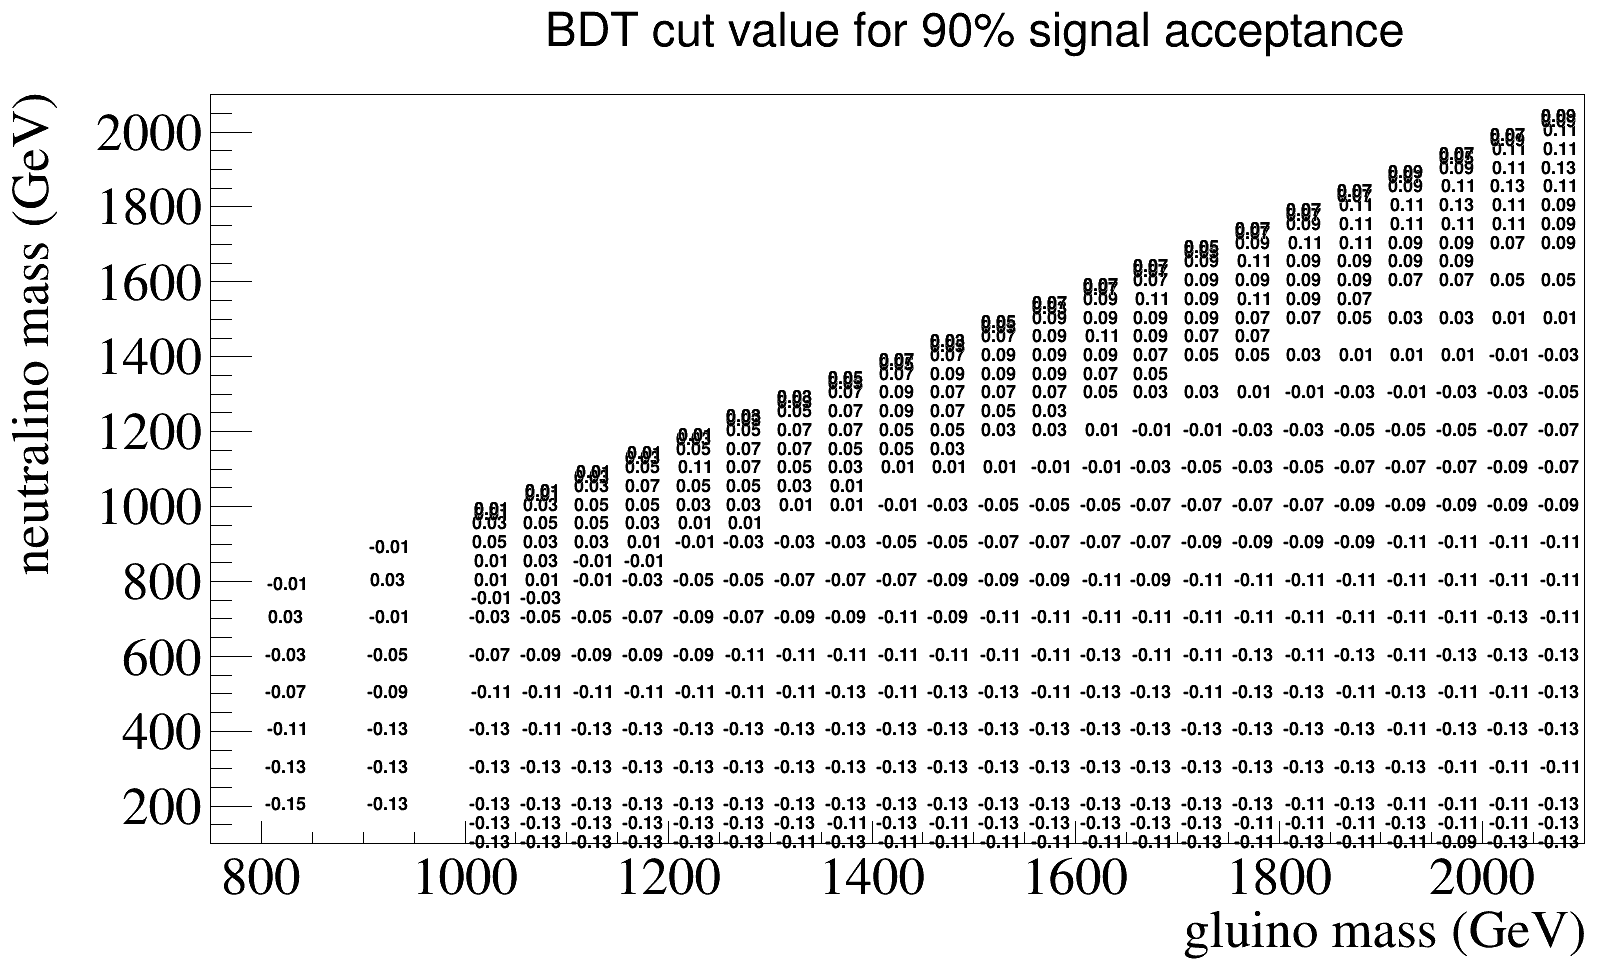
\includegraphics[width=1.5\linewidth,angle=90]{Figures/T5Wg_bdtcuts}
	\caption[BDT cut values on T5gg models resulting in 90\% signal acceptance.]{BDT cut values on T5gg models resulting in 90\% signal acceptance.}
	\label{fig:t5wgbdtcuts}
\end{figure}
\begin{figure}[h]
	\centering
	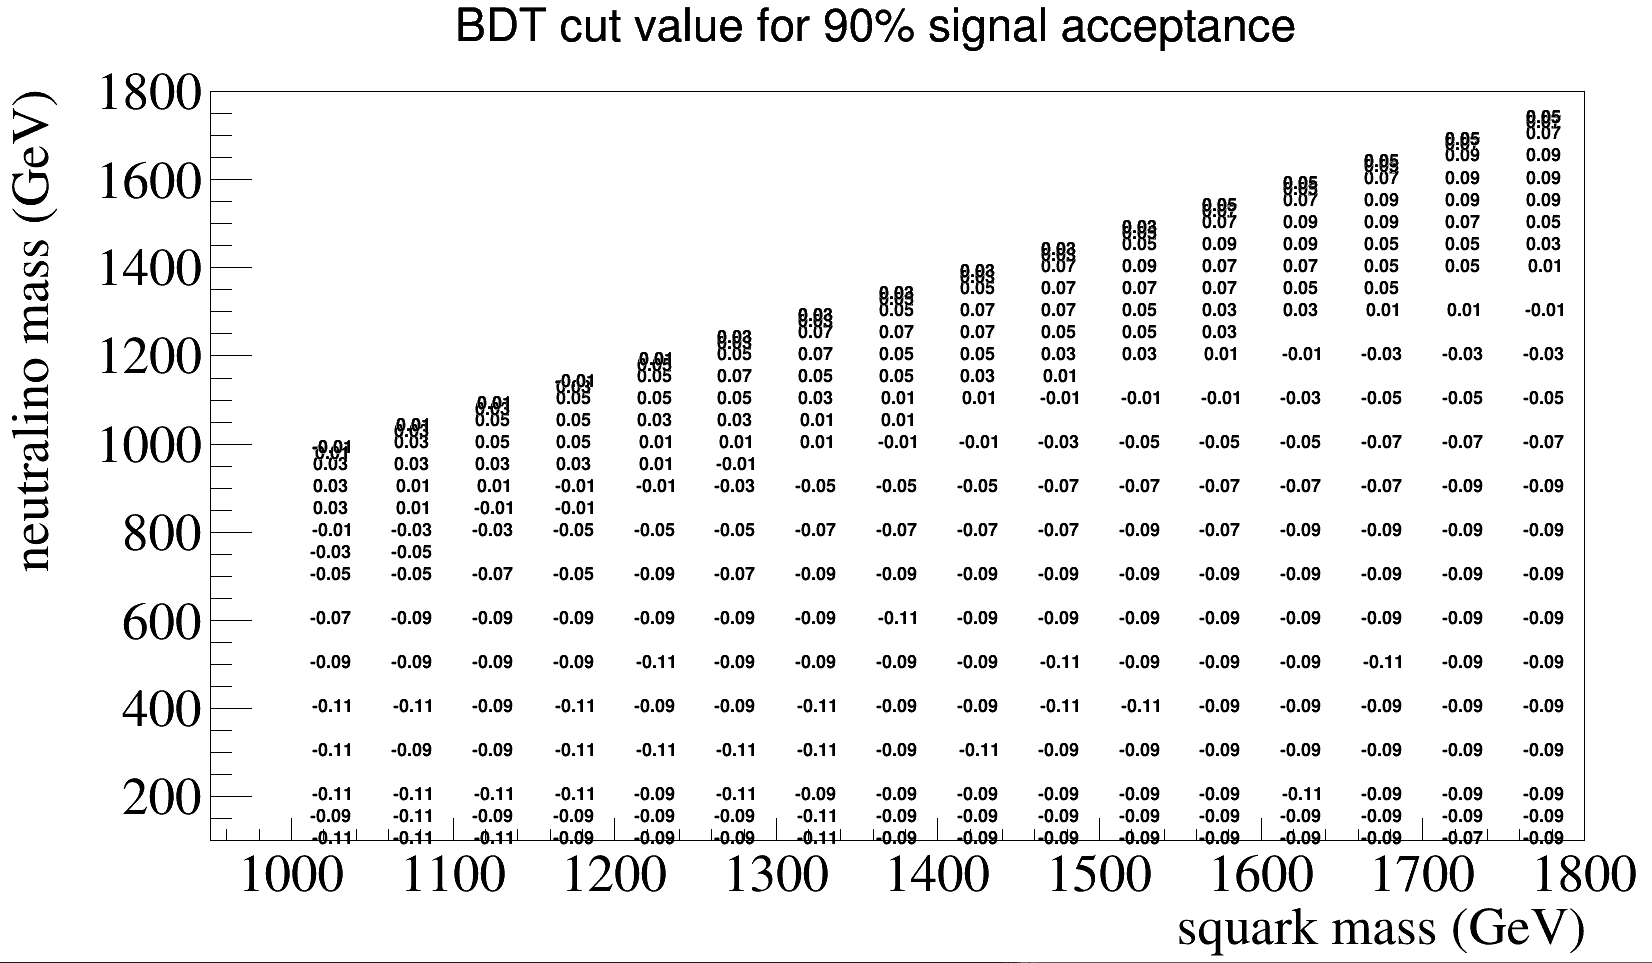
\includegraphics[width=1.5\linewidth, angle=90]{Figures/T6Wg_bdtcuts}
	\caption[BDT cut values on T6gg models resulting in 90\% signal acceptance.]{BDT cut values on T6gg models resulting in 90\% signal acceptance.}
	\label{fig:t6wgbdtcuts}
\end{figure}
\begin{figure}[h]
	\centering
	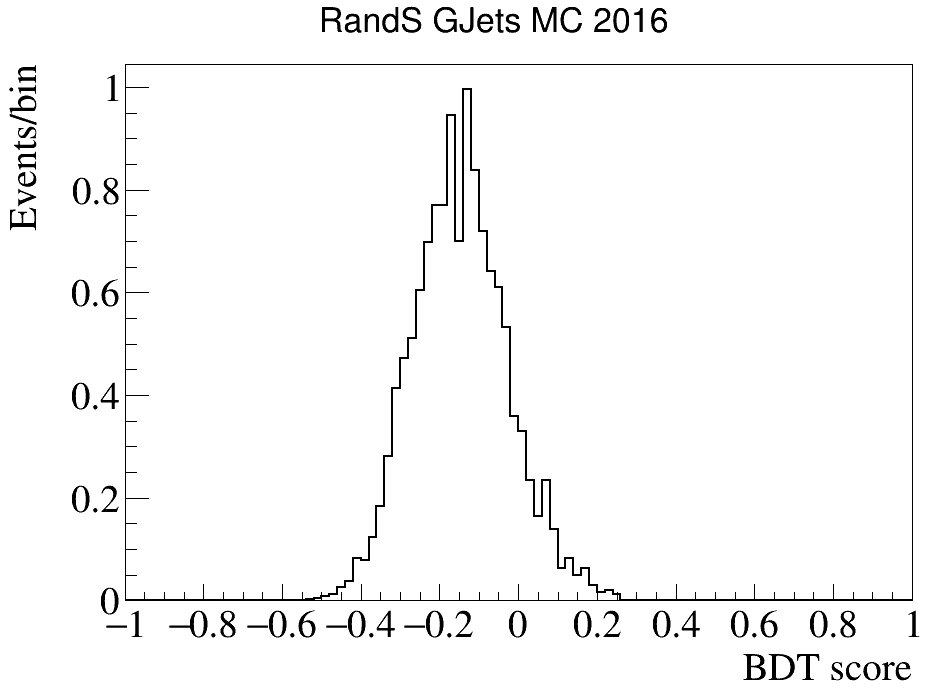
\includegraphics[width=0.7\linewidth]{Figures/GJets_BDT_2016}
	\caption[BDT response to Rebalance and Smear events in 2016 GJets MC]{This is the BDT score distribution for Rebalance and Smear events from the 2016 GJets MC samples. Requiring a BDT score above 0.03 removes 90\% of this background.}
	\label{fig:bdtgjets}
\end{figure}
\begin{figure}[h]
	\centering
	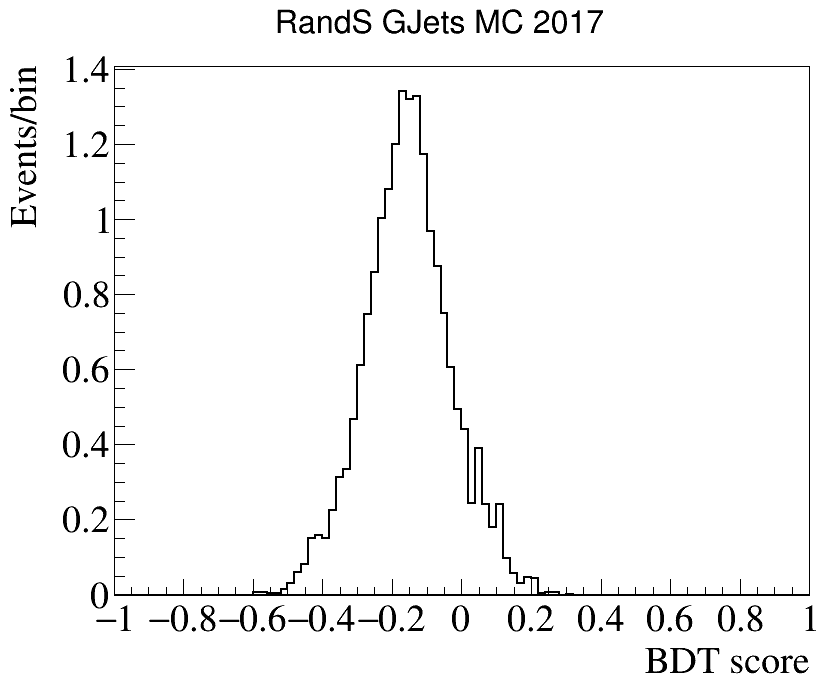
\includegraphics[width=0.7\linewidth]{Figures/GJets_BDT_2017}
	\caption[BDT response to Rebalance and Smear events in 2017 GJets MC]{This is the BDT score distribution for Rebalance and Smear events from the 2017 GJets MC samples. Requiring a BDT score above 0.03 removes 90\% of this background.}
	\label{fig:bdtgjets2017}
\end{figure}
\begin{figure}[h]
	\centering
	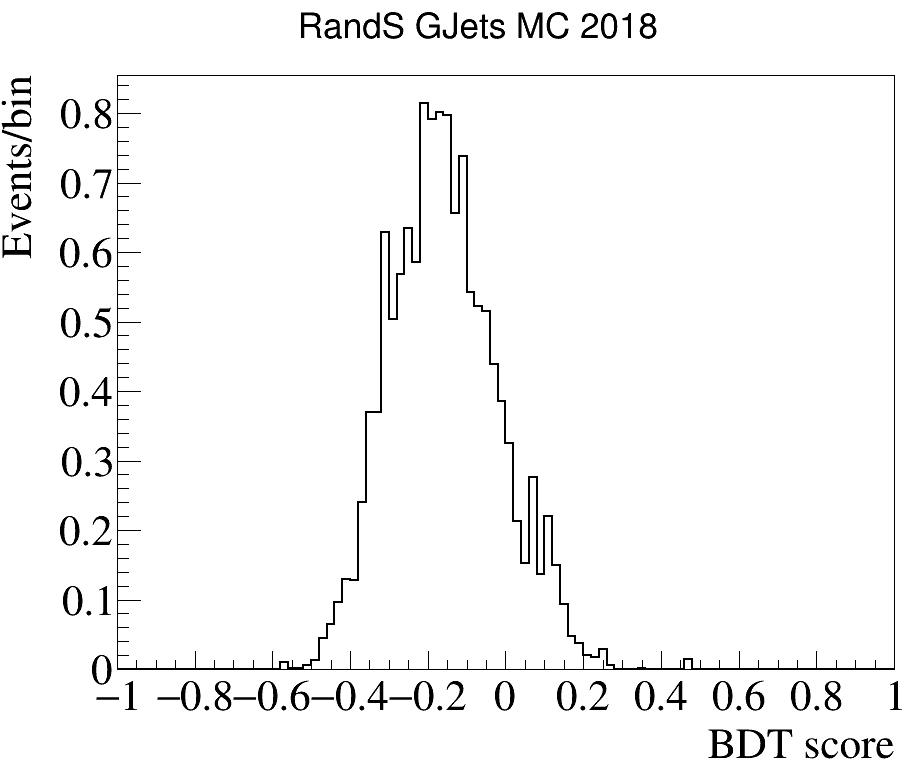
\includegraphics[width=0.7\linewidth]{Figures/GJets_BDT_2018}
	\caption[BDT response to Rebalance and Smear events in 2018 GJets MC]{This is the BDT score distribution for Rebalance and Smear events from the 2018 GJets MC samples. Requiring a BDT score above 0.03 removes 90\% of this background.}
	\label{fig:bdtgjets2018}
\end{figure}
%\begin{figure}[h]
%	\centering
%	\subfloat[T6GG mass grid with medium BDT cut values][T6GG mass grid with medium BDT cut values]{
%		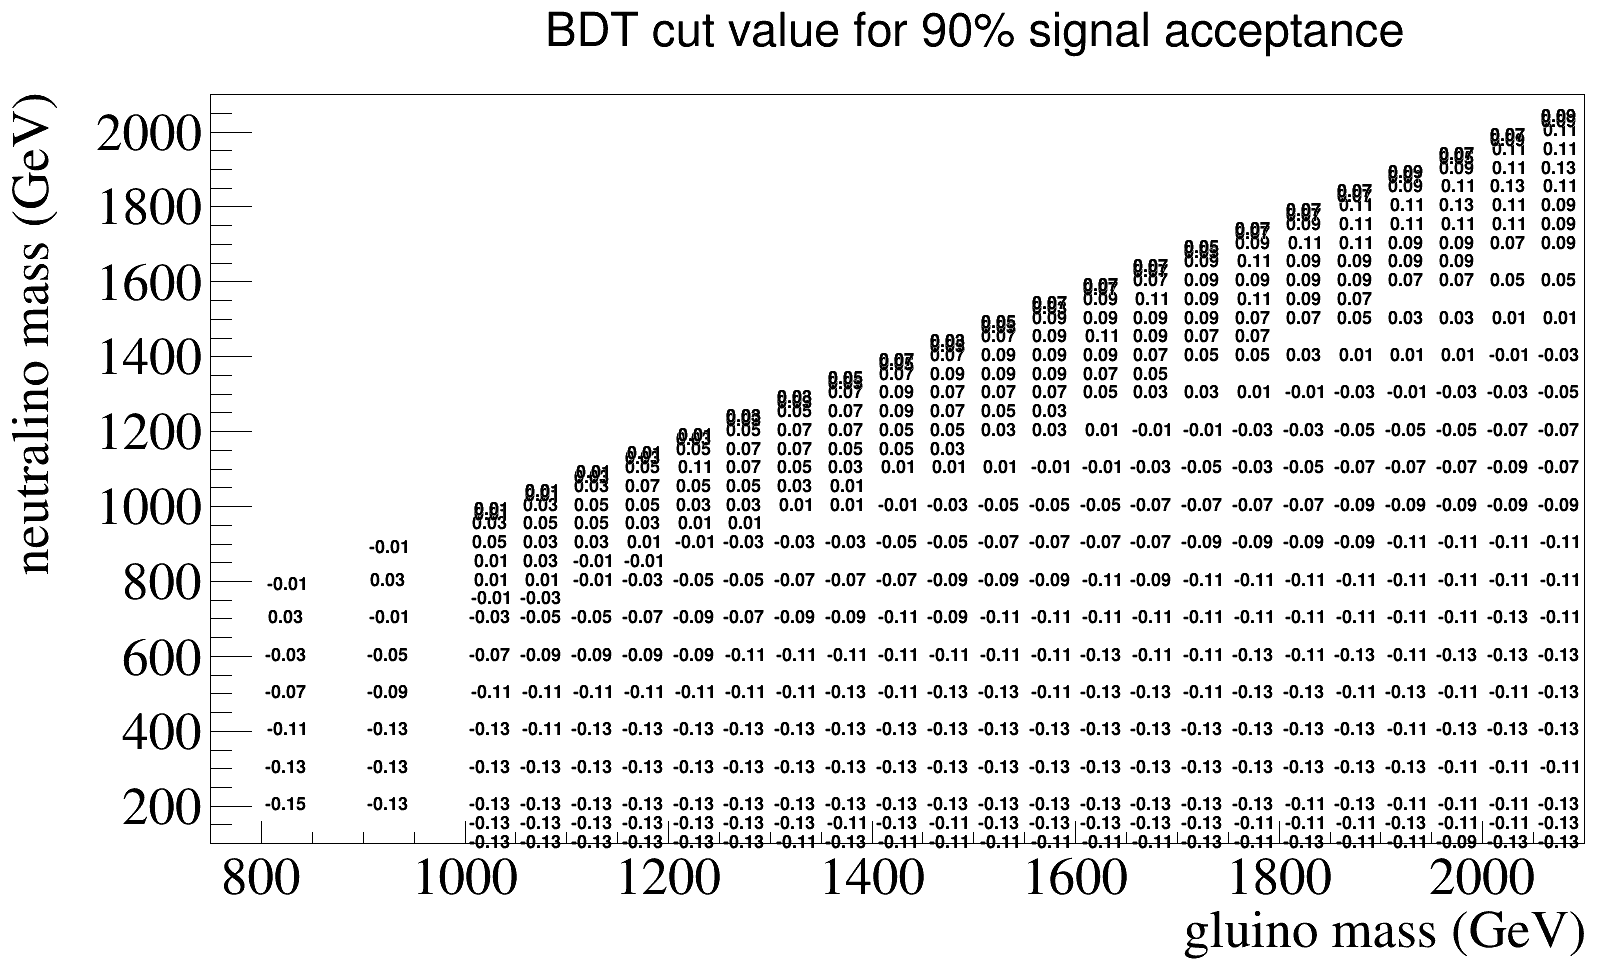
\includegraphics[width=1.1\textwidth]{Figures/T5Wg_bdtcuts}
%		\label{fig:T5bdtcuts}}
%	\qquad
%	\subfloat[T6GG mass grid with medium BDT cut values][T6GG mass grid with medium BDT cut values]{
%		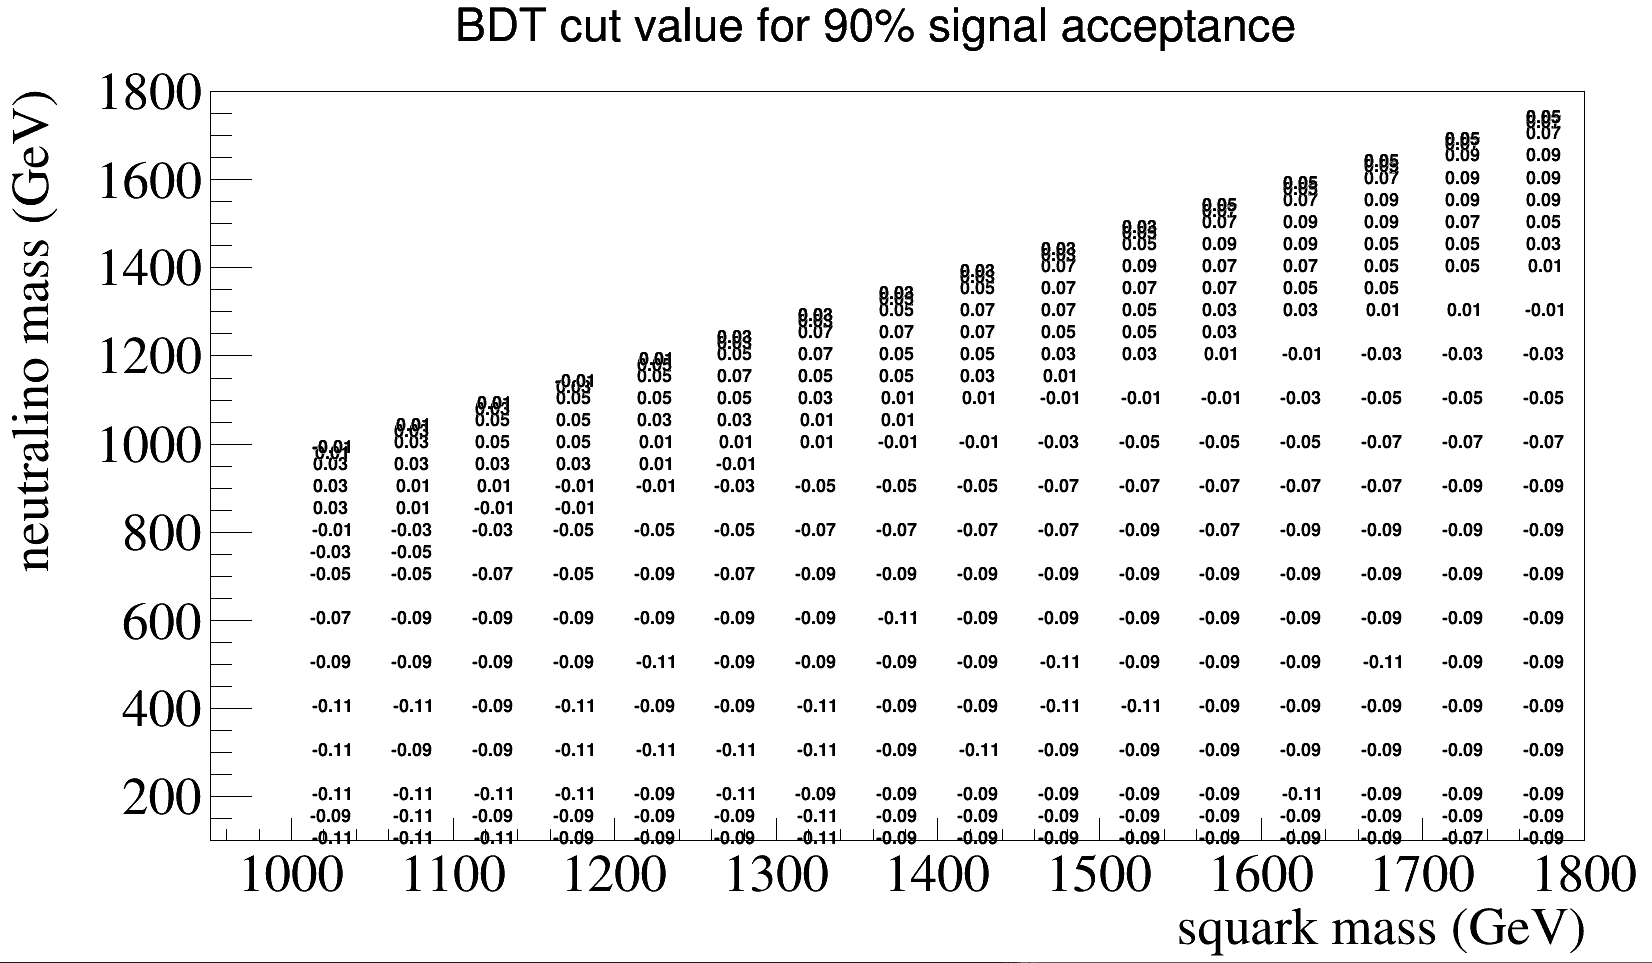
\includegraphics[width=1.1\textwidth]{Figures/T6Wg_bdtcuts}
%		\label{fig:T6bdtcuts}}
%	\caption{The mass grids for showing the minimum value of the BDT cut at each mass point that would give 90\% signal acceptance.}
%	\label{fig:bdtcuts}
%\end{figure}

\subsection{Electroweak background}
The electroweak background is dominated by events with $W \rightarrow e \nu$ where the electron is misidentified as a photon.  Unlike the QCD background these events have  real $E^{miss}_T$ due to the presence of a neutrino.  The key to estimating this background is determining the rate at which electrons get incorrectly labeled as photons in the signal region.  This is done using a tag-and-probe method where the tag is an electron (a loose ID photon that fails the PSV) and the probe is categorized as either a photon or an electron.  The result is an electron-electron region ($ee$) and an electron-photon region ($e\gamma$) that are selected from the data.    As both of these regions contain $Z\rightarrow ee$ decays, fits are applied in each of the samples to the invariant mass spectra $m_{ee}$ and $m_{e\gamma}$.  The integrals of these fits are calculated over the range of the Z mass peak to give the number of events in each category, $N_{e\gamma}$ and $N_{ee}$.  The ratio of the number of 


%This is done using two control regions.  The first is double electron ($ee$) region.  As described before, the electrons are defined as loose ID photons that have a pixel seed match.  The second is the $e\gamma$ region which contains one electron and one photon.  The misidentification rate can be calculated by comparing the invariant mass peaks $m_{ee}$ and $m_{e\gamma}$.  



\subsection{Irreducible background}
The irreducible $Z \gamma \gamma \rightarrow \nu \nu \gamma \gamma$ background produces two photons and has inherent $E^{miss}_T$ via the neutrinos.  There is no easy way to separate these events from our signal so it is estimated using MC simulation.  The prediction of this background is given by $N_{pred} = N_{MC}\cdot R$ where $R$ is an overall simulation-to-data normalization factor obtained by comparing $Z \gamma \gamma \rightarrow LL \gamma \gamma$ MC samples to $Z\gamma \gamma \rightarrow \mu \mu \gamma \gamma$ and $Z\gamma \gamma \rightarrow ee \gamma \gamma$ events in data.  The event selection criteria, relaxed from the baseline version in order to maximize statistics, was
\begin{itemize}
	\item 2 looseID photons with $p_T$ > 30 GeV and no pixel seed
	\item 2 like-flavored leptons with $p_T$ > 30 GeV %and $|m_{LL} - m_Z|<10$ GeV
	\subitem 2 mediumID muons or
	\subitem 2 electons (looseID photons with pixel seeds).
\end{itemize}
The resulting dilepton invariant mass spectra for 2016 MC and data are shown in Figure \ref{fig:zggtonunugg2016fullmass}.  The number of events with dilepton mass within 10 GeV of the Z boson mass is shown in Table \ref{table:ZGGtonunuGG}.  The ratio of data events to MC events gives the normalization factor $R$ factor which was applied to the $Z \gamma \gamma \rightarrow \nu \nu \gamma \gamma$ MC to give the background prediction for this process.

%The appropriate scale factors were applied for the photons, muons, and electrons in the MC samples.  The resulting dilepton invariant mass spectra for 2016 MC and data are shown in Figure \ref{fig:zggtonunugg2016fullmass}.  The number of events with dilepton mass within 10 GeV of the Z boson mass is shown in Table \ref{table:ZGGtonunuGG}.  The ratio of data events to MC events gives a scale factor which was applied to the $Z \gamma \gamma \rightarrow \nu \nu \gamma \gamma$ MC to correct for the difference in normalization resulting from mismodeling of this background.

\begin{figure}[h]
	\centering
	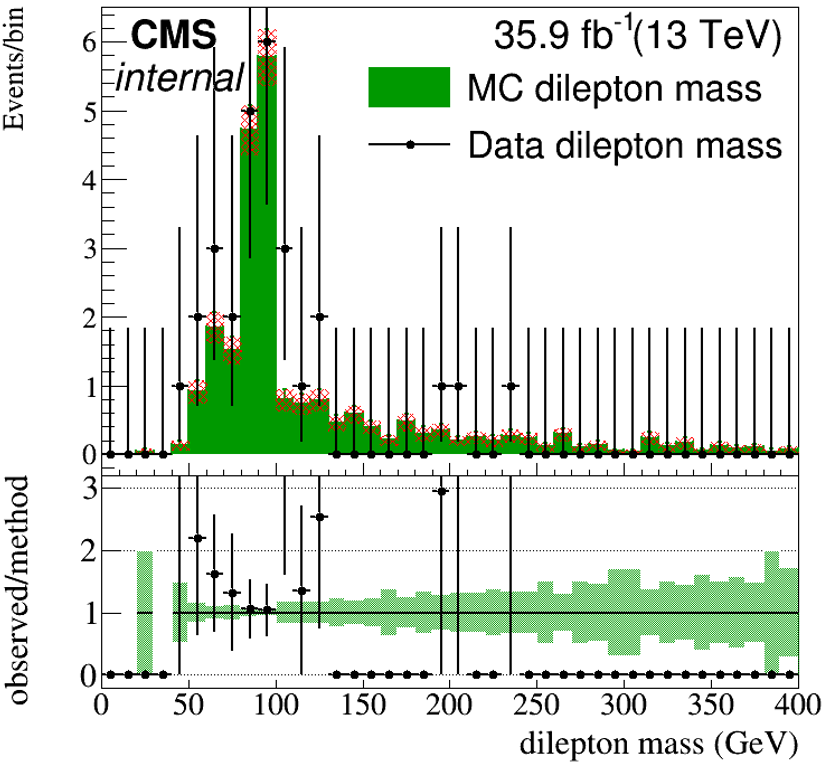
\includegraphics[width=0.7\linewidth]{Figures/ZGGtonunuGG_2016_fullmass}
	\caption[Comparison of ZGGToLLGG MC to data]{Comparison of dilepton invariant mass spectra from ZGGToLLGG events in MC and data.  Good agreement is seen in the region where the invariant mass is within 10 GeV of the Z boson mass (91 GeV).}
	\label{fig:zggtonunugg2016fullmass}
\end{figure}




%The modeling of this background was tested using $Z\gamma \gamma \rightarrow \mu \mu \gamma \gamma$ and $Z\gamma \gamma \rightarrow ee \gamma \gamma$ events in data.  Di-muon events with $|m_{\mu \mu} - m_Z|<15$ GeV and di-electron events with $|m_{ee}-m_Z|<15$ GeV were selected and the contribution of the muons/electrons was removed from the $E^{miss}_T$ calculation to mimic $Z\rightarrow \nu \nu$.  The event selection criteria for this $Z \gamma \gamma \rightarrow LL \gamma \gamma$ control region was

%The relationship
%\begin{equation}
%	N_{Z\rightarrow \nu \nu} = \frac{b_{Z\rightarrow \nu \nu}}{b_{Z\rightarrow ee}+b_{Z\rightarrow \mu \mu}}(N_{Z\rightarrow ee}+N_{Z\rightarrow \mu \mu})
%	\label{equation:zggtonunugg}
%\end{equation}
%gives an estimation for the number of $Z \gamma \gamma \rightarrow \nu \nu \gamma \gamma$ events expected given the number of $Z \gamma \gamma \rightarrow LL \gamma \gamma$ events observed in data where $N_{Z\rightarrow ee}$ and $N_{Z\rightarrow \mu \mu}$ are the number of data events passing the aforementioned selection criteria and $b_{Z\rightarrow \nu \nu}$, $b_{Z\rightarrow \mu \mu}$, and $b_{Z\rightarrow ee}$ are the branching ratios.  The results are summarized in Table \ref{table:ZGGtonunuGG}.

\begin{table}[h]
	\centering
	\caption{Summary of $Z \gamma \gamma \rightarrow \nu \nu \gamma \gamma$ model validation}
	\begin{tabular}{|l|l|l|l|}
		\hline
		Year & Data Events & MC Events & $R = \frac{data}{MC}$ \\
		\hline
		\hline
		2016 & 10.0 +4.78 -3.05 & 10.54 $\pm$0.54 & 0.95 +0.46 -0.29 \\
		\hline
		2017 & - & - & - \\
		\hline
		2018 & - & - & - \\
		\hline
	\end{tabular}
	\label{table:ZGGtonunuGG}
\end{table}

\section{Signal and control regions}
The background estimation methods are validated in various low-BDT data control regions.  

The first such region is the low-BDT $ee$ region in which the pixel seed veto requirements are inverted, resulting in events with two electrons.  This region is primarily composed of $t\bar{t}$, which is a source of real $E_T^{miss}$, and Drell-Yan (DY) with $Z\rightarrow ee$.  As the DY background is comprised of multi-jet events with two electrons (photos with inverted pixel seed requirements), this is a source of fake $E_T^{miss}$ that is very similar yet orthogonal to our expected signal which consists of multi-jet events with two photons.